\documentclass[oneside]{article}
\usepackage{fullpage}
\usepackage[pdftex]{graphicx}
\DeclareGraphicsExtensions{.png,.pdf}
\graphicspath{{images/}}
\usepackage{hyperref}
\usepackage{verbatim}
\usepackage[format=plain,font=small]{caption}
\usepackage[small]{titlesec}
\usepackage[round,sectionbib]{natbib}
\usepackage{amstext}
\bibliographystyle{plainnat}
\renewcommand\rmdefault{bch}
\linespread{1.07} 

\newcommand\amin{\text{minor}}
\newcommand\amaj{\text{major}}

\begin{document}

\title{Glyph-maps for visualizing climate data and models}
\author{Cook, Hofmann, Wickham, Wickham}

% Found data: http://www.esrl.noaa.gov/psd/data/gridded/data.HADCRUT2.html
%     air.mon.anom.nc, var adj, this is 5x5 degree grid, a bit sparse
% Or: http://www.esrl.noaa.gov/psd/data/gridded/data.gisstemp.html
% air.2x2.mon.anom.land.nc 250k smooth data, is on a 2x2 grid

% Drawing trend lines on map
%   - How to
%   - Comparison to coloring slope
%   - Reference to Grinstein icon plots
% Pickett RM and Grinstein GG (1988). Iconographics 
% displays for visualizing multidimensional data. 
% In Proc. IEEE Conference on Systems, Man, and Cybernetics, pages 514-19.
% Note the later work on metaphoric data display, garbage work!
%   - Alexander Gribov's work http://rosuda.org/software/Gauguin/gauguin.html

%   - Spatial star plots by Andrews http://www.udallas.edu:8080/~andrews/software/software.html
%   - Look at what Bertin does
%
% Interactive graphics
% Data processing
%
% Perhaps the GHCN data? Not gridded
% NOAA data, almost grid, but over ocean, so maps more tricky
% NARCAP from NCAR?
% Fill in with NASA data, to start, try to put new data for final version
\maketitle

\section{Introduction}

Climate data is composed of measurements on variables such as temperature, precipitation, and winds that have been collected from a spatial and temporal context. The classic display for spatial data is to use color or grey scale overlaid on geographic location, typically including a map. When measurements are made at different time periods it is common to display the data as small multiples, such as in Figure \ref{fig:facetted-map}. In this plot, a separate map is drawn for each month (columns) and year (rows), over a 6 year period of remotely sensed temperature data above Central America. Color is used to display the de-seasonalized temperature measurements, with red being high values and blue being low values. The data comes from \citet{murrell:2010}. The most noticeable feature in this display is the strong red in the equatorial region beginning in mid-1997 and tapering out during 1998. This is the pattern of an El Ni\~no event, a major temperature anomaly. With some work other smaller more localized patterns can be perceived, for example, cooler over the land mass in the early year, but warmer in the latter years. What the reader is required to do is play the game ``Spot the difference'' from one small image to another. From a cognitive perspective, this is a very hard task to do. It falls into the framework of {\it change blindness} (see e.g. \citet{healey:2011} and often leads to failure without readers realizing, in particular for small areas of change or subtle changes.  Large structures such as the El Ni\~no event are clear but readers will not be able to effectively glue the images together sufficiently to read off the trend over the years or notice small local deviations between plots. Rendering these small multiples as movie helps with picking up strong trends, but small trends still fail to draw readers' attention and escape unnoticed \citep{simons:gradual}.

\begin{figure*}[htp]
\centerline{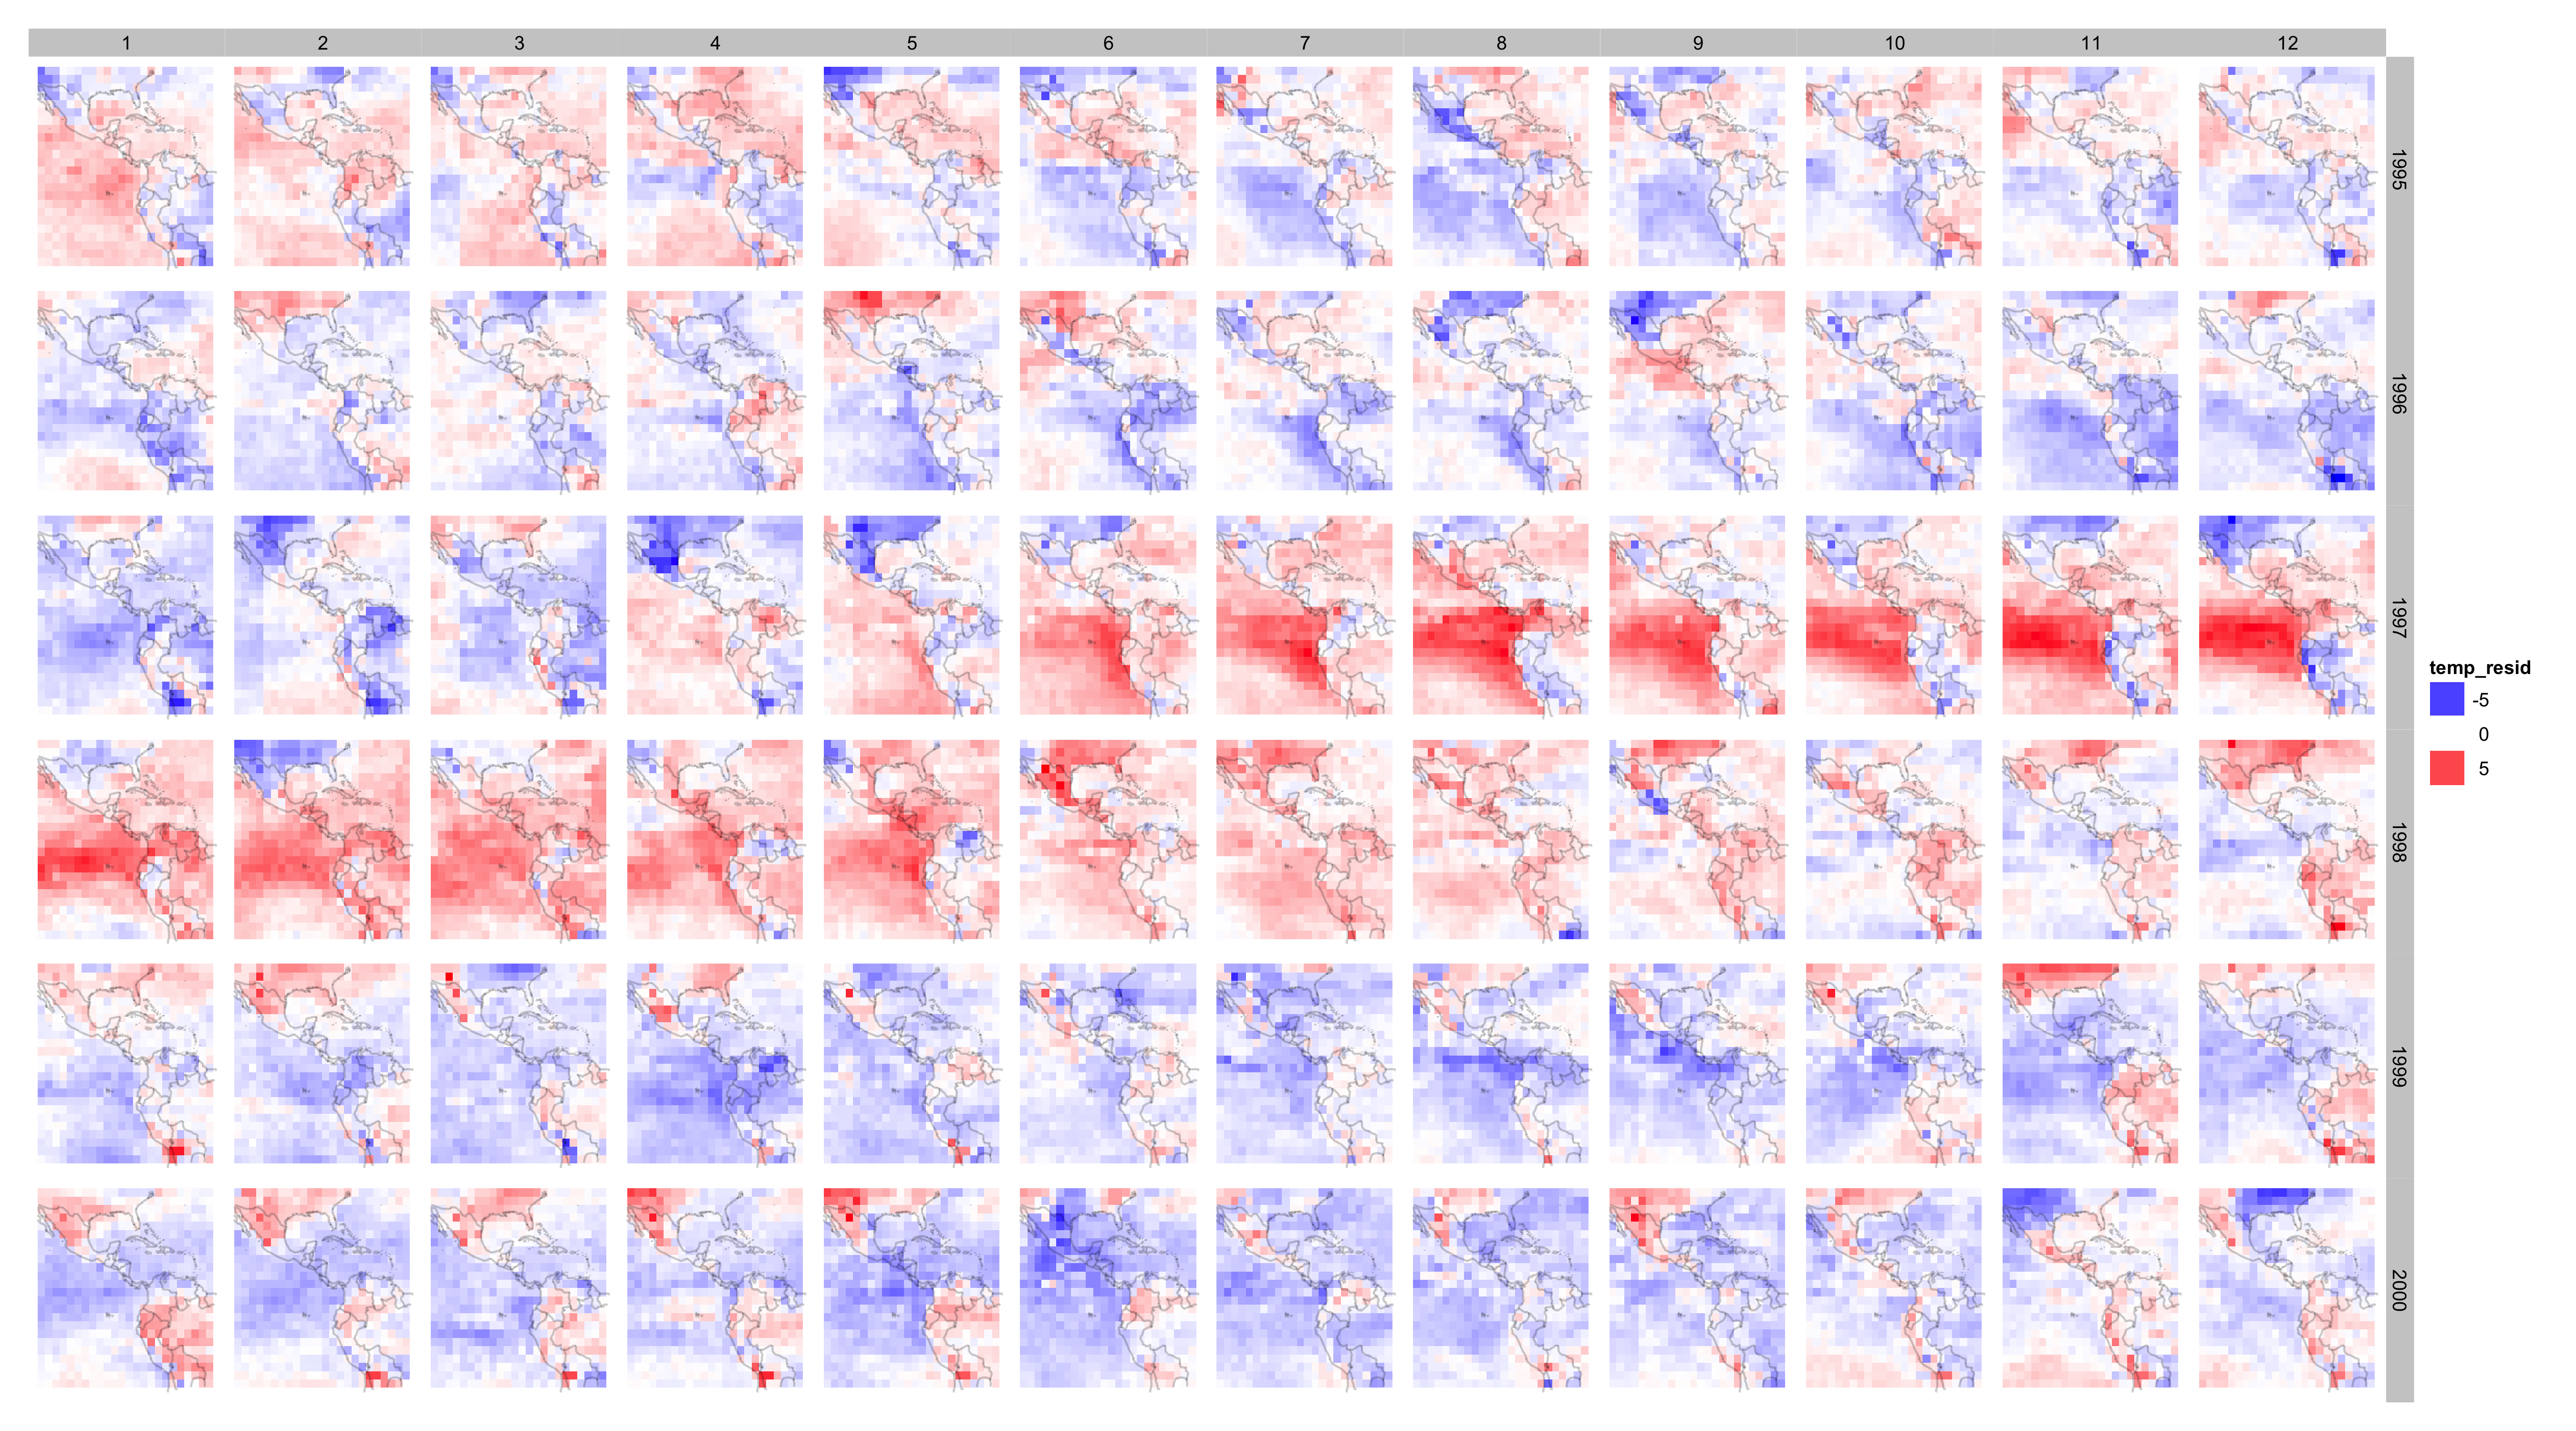
\includegraphics[width=6in]{nasa-colored-map.png}}
\caption{Facetted map of de-seasonalized temperature. The dominant feature is the El Ni\~no warming in the qouthern equatorial region in the last half of 1997 and first half of 1998. Smaller features are only noticeable on closer inspection, or if pointed out: such as the relative warming on the mountain regions in south and north America in the later years.}
\label{fig:facetted-map}
\end{figure*}

%% Reproduce all of the icon displays using the fixed glyph code

In this paper we explore the use of a different type of display, that uses icons on the map, for climate data.  Icon plot associated with weather maps date back as far as \citet{galton:weathermap}, described in \citet{friendlydenis:2001}. Icon plots date back to the star plot introduced by \citet{mayr:1877}, and resurged in the modern era with the semi-graphic displays of \citet{anderson:1960}, and were made infamous by \citep{chernoff:1973}. An icon is produced by mapping each variable to some feature of the icon. One icon is generated for every case in the data set. %Figure \ref{fig:glyphs} illustrates the construction of star plot, with emphasis on temporal data. 
For temporal data, time measurements can be treated as variables in a multivariate data set, fitting this into the icon plot framework. Figure \ref{templates} displays 12 iconic time series shapes, and how they would look if the icon was a time series, or displayed as a star glyph. The data underlying each glyph has 36 time variables. The star glyphs is formed by considering the 36 axes radiating from a common midpoint, and the data values for the row are plotted on each axis relative to the locations of the minimum and maximum of the variable. For the temporal data, all variables are considered to be on a common scale so the global minimum and maximum of temperature are used to scale each data value. 
%Three different locations are selected, for demonstration purposes. The top plot shows the time series of these three locations. Location ``1.1'' (red) has medium values of temperature, with strong seasonality, the six years corresponding to the six peaks. Location ``2.1'' (green) has generally high temperature values, with weaker seasonality in most years and a lack of low temperatures in the middle of the time period when lows would be expected. Location ``3.1'' (blue) has strong seasonality but generally low temperatures. The bottom plot shows these same cases as star glyphs. A separate glyph is created for each location. The 72 time variables form axes organized radially. Each temperature value is plotted relative to the overall range of temperature values. The seasonal patterns are clearly visible in this type of display, forming six ``petals'' in the icon. Location ``2.1'' has a different pattern than the other two, with only four petals, and location ``3.1'' is a much smaller icon indicating overall lower values. 

\begin{figure}[htbp]
  \centering
  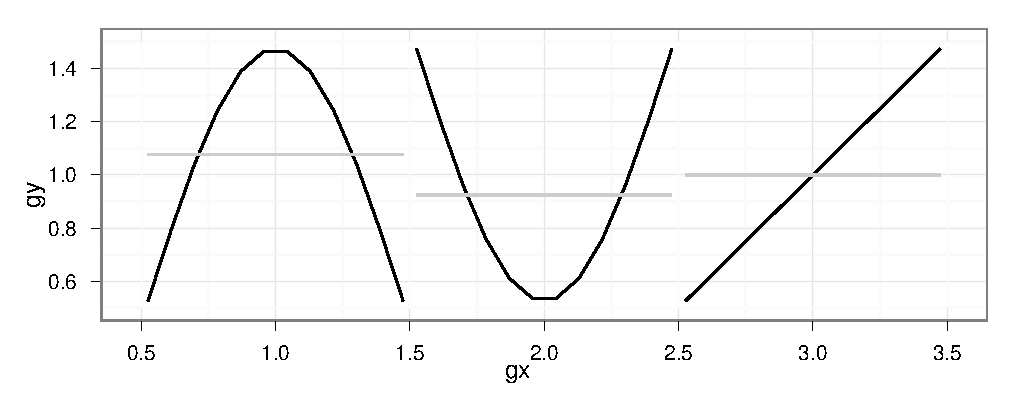
\includegraphics[width=0.5\linewidth]{euclid-to-polar-1}%
  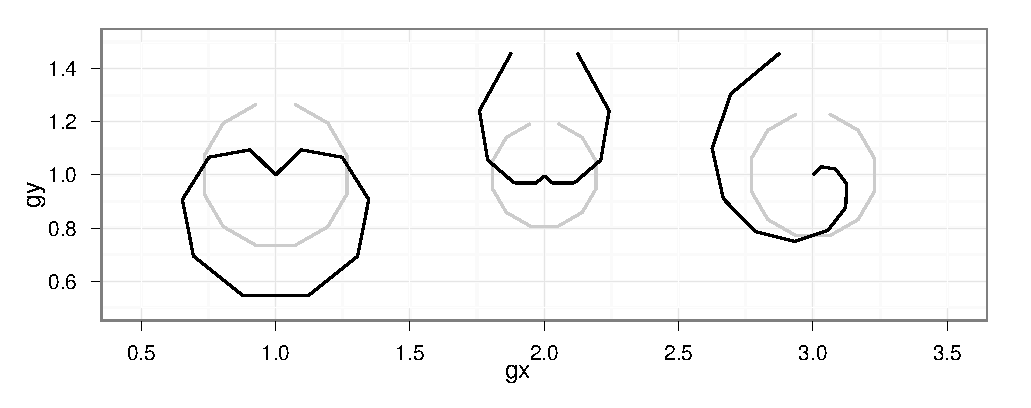
\includegraphics[width=0.5\linewidth]{euclid-to-polar-2}

  \caption{Icon plots for 12 iconic time series shapes (linear increasing, decreasing, shifted, single peak, single dip, combined linear and nonlinear, seasonal trends with different scales, and a combined linear and seasonal trend) in Euclidean coordinates, time series icons (left) and polar coordinates, star plots (right).}
  \label{fig:templates}
\end{figure}


%\begin{figure*}[htp]
%\centerline{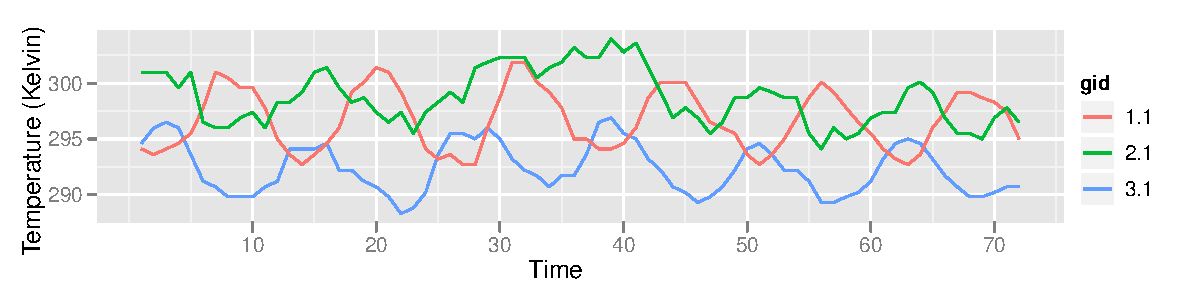
\includegraphics[width=6in]{nasa-glyph-ts.pdf}}
%\centerline{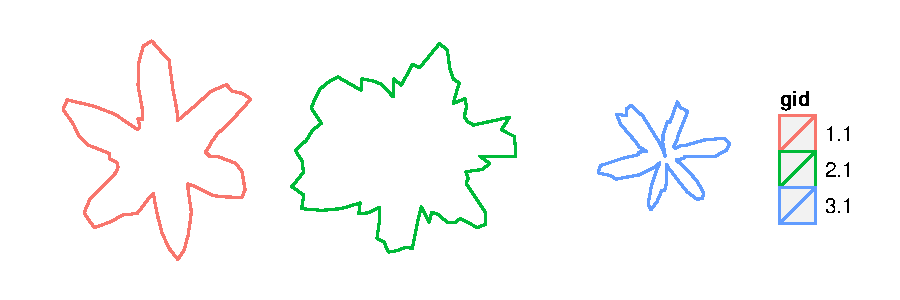
\includegraphics[width=6in]{nasa-glyph.pdf}}
%\caption{Icons of raw temperature for three different locations.}
%\label{fig:glyphs}
%\end{figure*}

Icon plots are used, infrequently, to examine multivariate data. For large data sets it is infeasible to digest the quantity of icons, and for multivariate data there is no natural order so it can be like having a mountain of little stamps to rearrange and organize, in order to understand the structures present in the data. An early paper on multivariate graphics \citep{kleiner:1981} and a recent paper \citep{hurley:2010} propose some approaches for organizing the icons. Ordering of icons is not an issue with spatiotemporal data, because it is naturally handled by spatial location. The spatial trend, or continuity, usually gives the plot an appearance of texturing on a landscape, make it easier to digest patterns among the icons.

In this paper we describe the algorithm for creating glyphs of temporal data on maps, generally in R, and the various modifcations that can enable different features in the data to be detected. The next section (\ref{sec:glyph-map}) describes the use of glyphs on maps, and Section \ref{sec:construction} explains how to construct glyph-maps. Section \ref{sec:reference} discusses the use of reference lines and boxes, and Section \ref{sec:scale} visits issues of scaling values for different information purposes. Generalizations to different types of icons are described in Section \ref{sec:scatter}. Glyph-maps work nicely with gridded data, but many spatiotemporaral data sets have irregular spatial locations. Possible adjustments are discussed in Section \ref{sec:irregular}. Code and data is available in the online supplementary materials.

\section{Glyph-maps}~\label{sec:glyph-map}

% Reference Tufte's small multiples
\emph{Glyph-maps} are maps where a glyph is displayed at each spatial location to represent multiple data values. To explain the glyph-map, we use data of 2$^o$x2$^o$ gridded temperature anomalies, from the GISTEMP surface temperature data provided by the Earth System Research Laboratory, Physical Sciences Division, National Oceanic and Atmospheric Administration. Ground station data was de-seasonalized, differenced from ***, and spatially averaged to obtain gridded measurements. Figure \ref{fig:gistemp-pred} shows the time series icons for each spatial location of predicted temperature for 1950-2010 across the USA. Most locations observe an increasing temperature, to varying degrees, over this time period. A few locations show a decline. These locations tend to be different from their neighbors, which might suggest isolated data problems. There is a difference in the temperature increase at different regions: steeper inclines can be seen in the north and western mountain region and across the Great Lakes, but inclines are flatter in the southeastern USA. 
%The most seasonality occurs in north American. Some seasonal effects can also be seen in the Caribbean and in south American locations. Around the equator the temperatures are relatively warm for all seasons. Instead of radially displaying the temperature a glyph can be a regular time series, time displayed horizontally and temperature vertically (right plot). The structure perceived is different with this change in glyph type: locations at the equator have flat series, on land more varied temperatures. 

\begin{figure}[htbp]
  \centering
  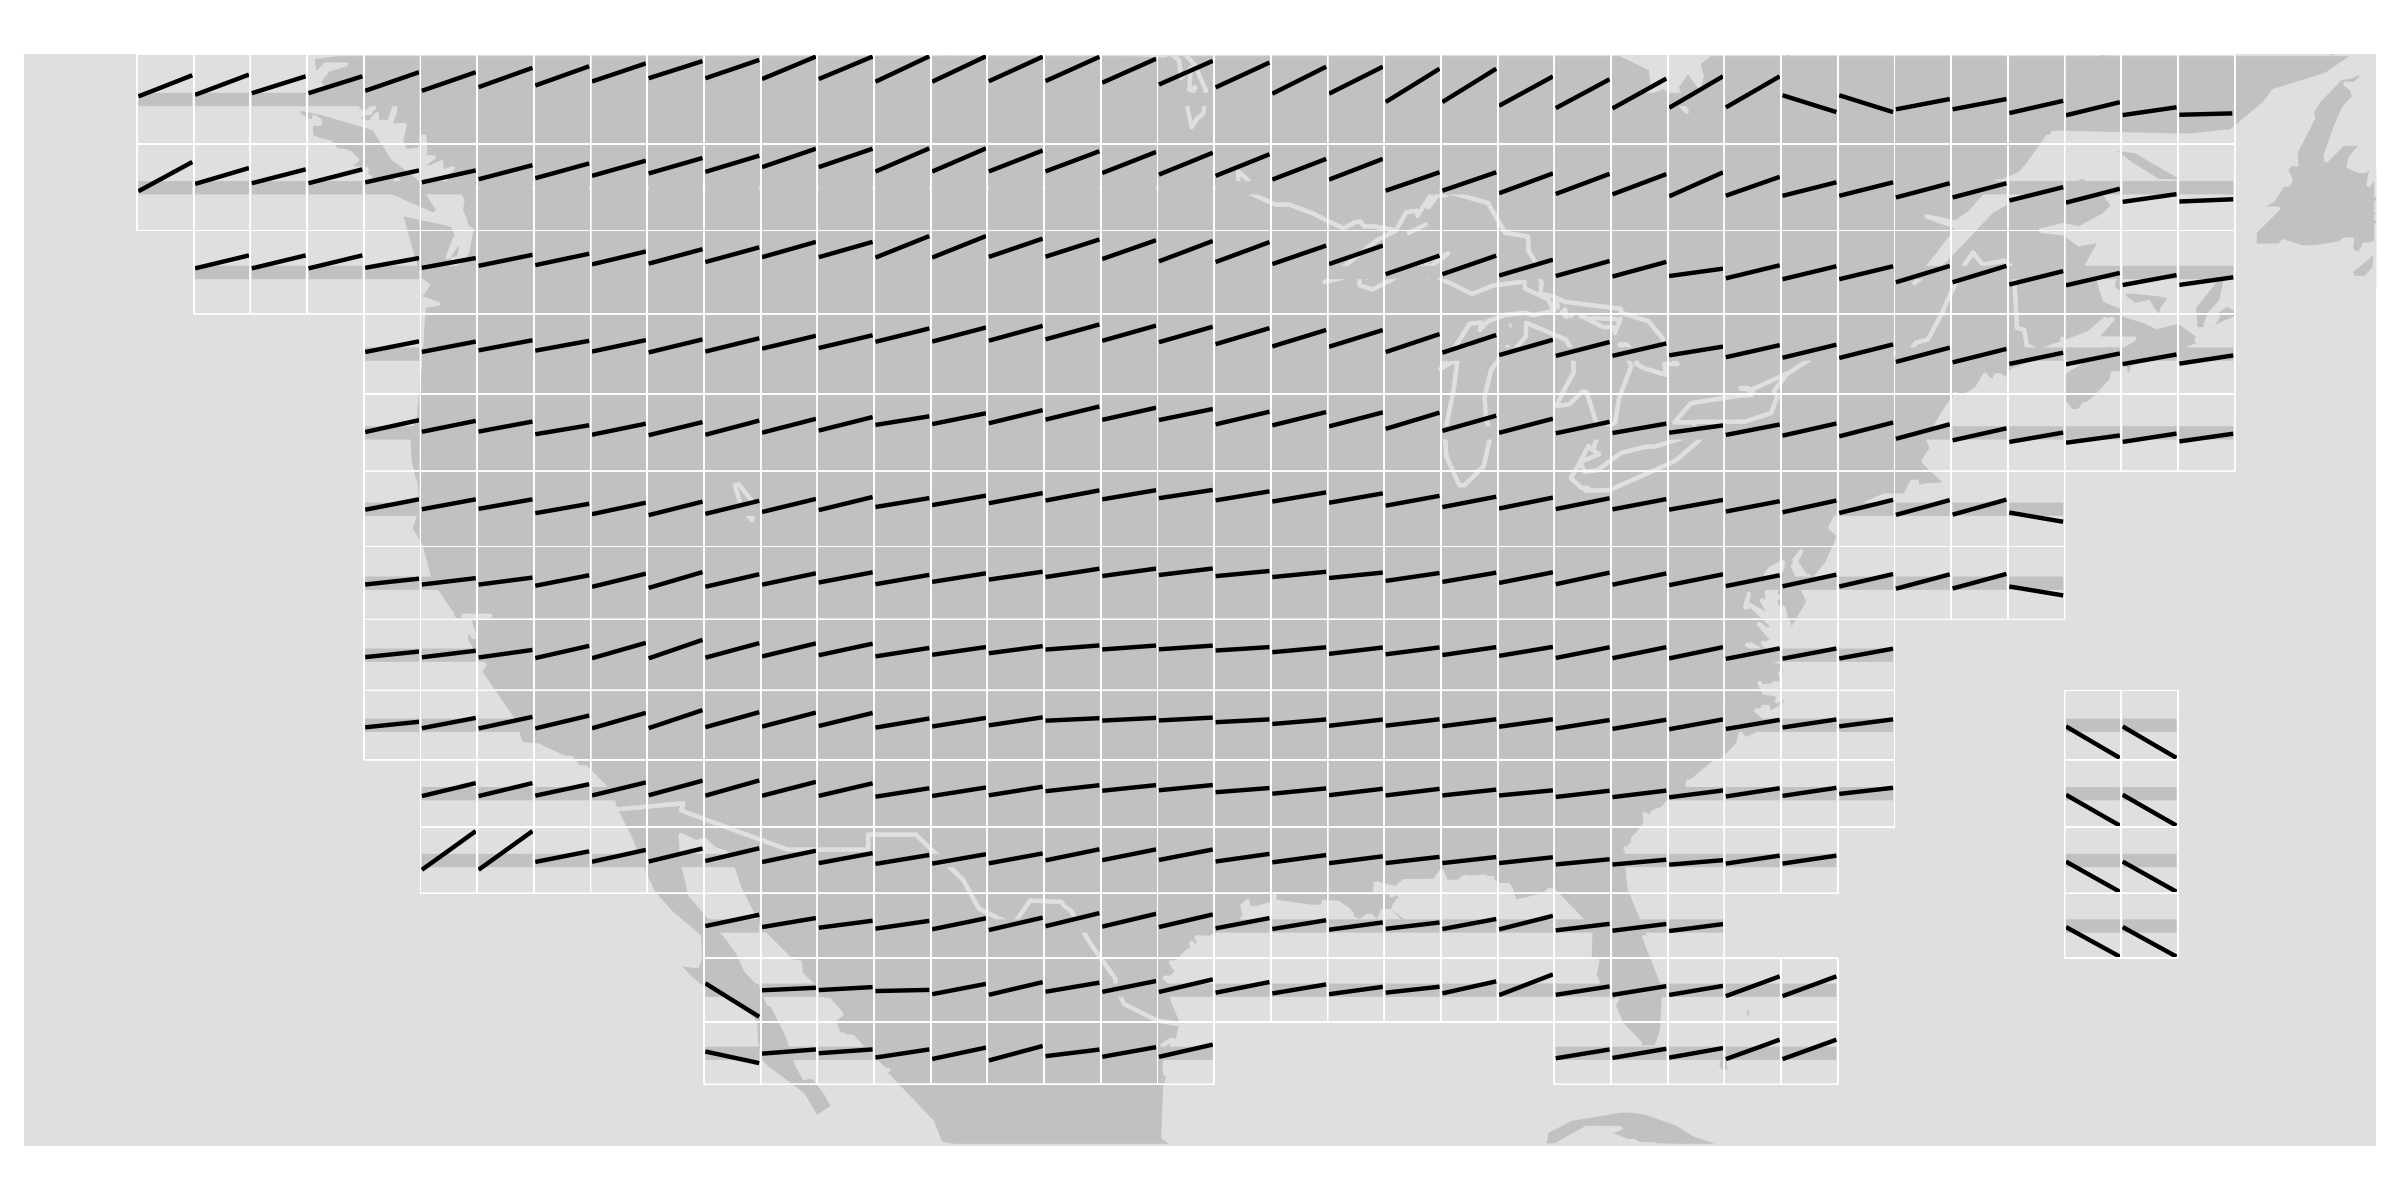
\includegraphics[width=1\linewidth]{gistemp-pred}%

  %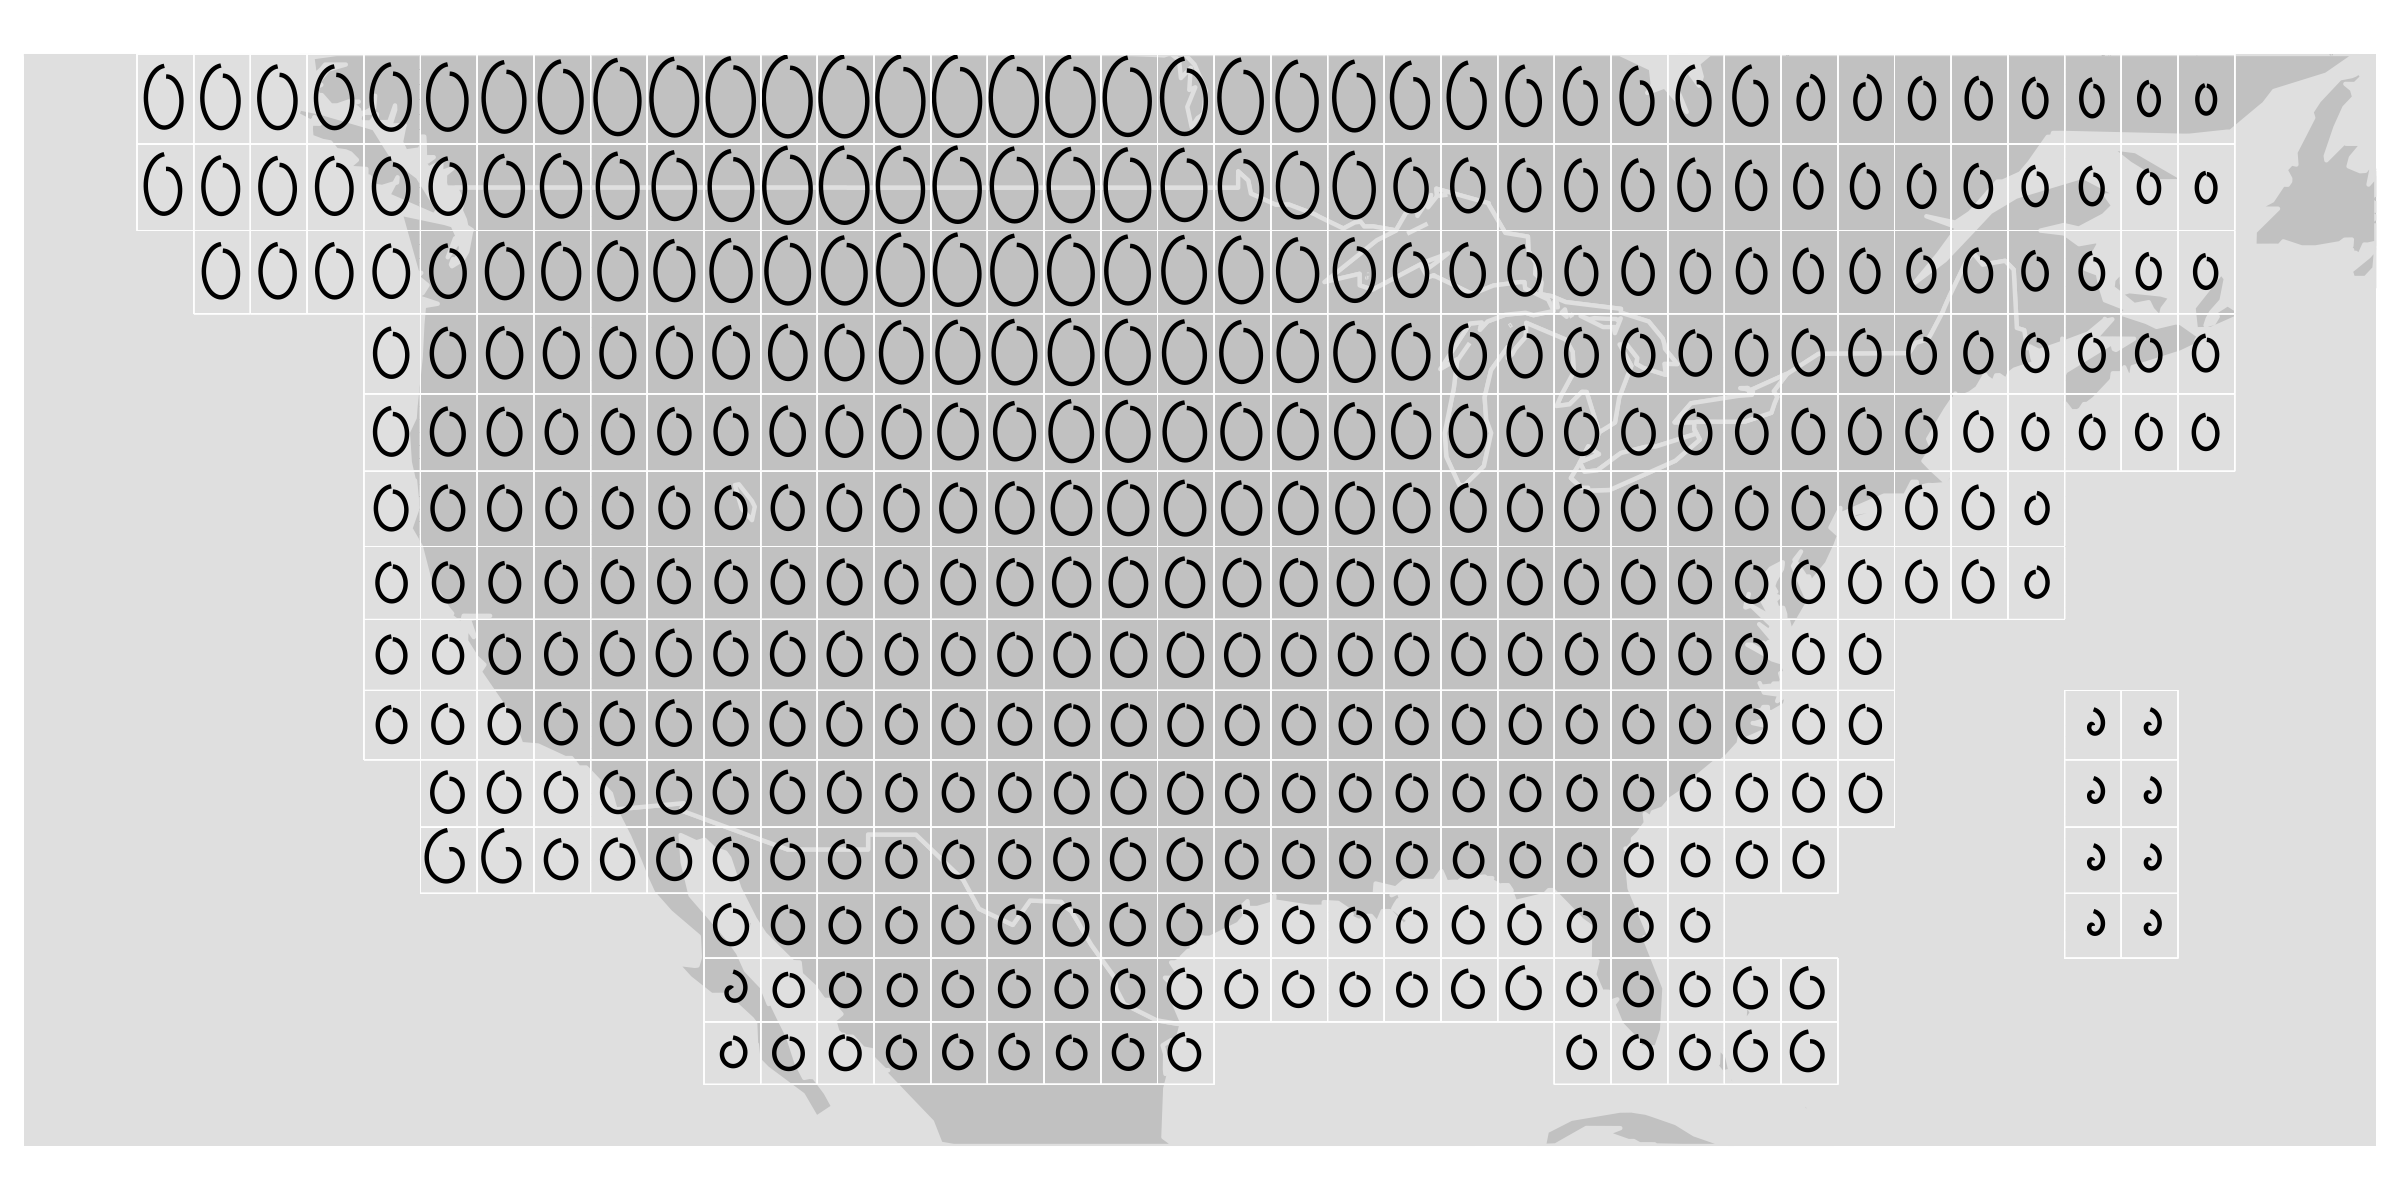
\includegraphics[width=1\linewidth]{gistemp-polar-pred}

  \caption{Glyph-map of predicted temperature anomaly data, from
    1950-2010. Increasing trends can be seen over most of the USA,
    with varying degrees of increase. Some isolated locations exhibit
    steep declines, and inclines, perpahs indicative of some isolated
    data problems.}
  \label{fig:gistemp-pred}
\end{figure}

*** Remove the strange data over ocean, and make the reference lines white?

% Add time series as well as radial
%\begin{figure*}[htp]
%\centerline{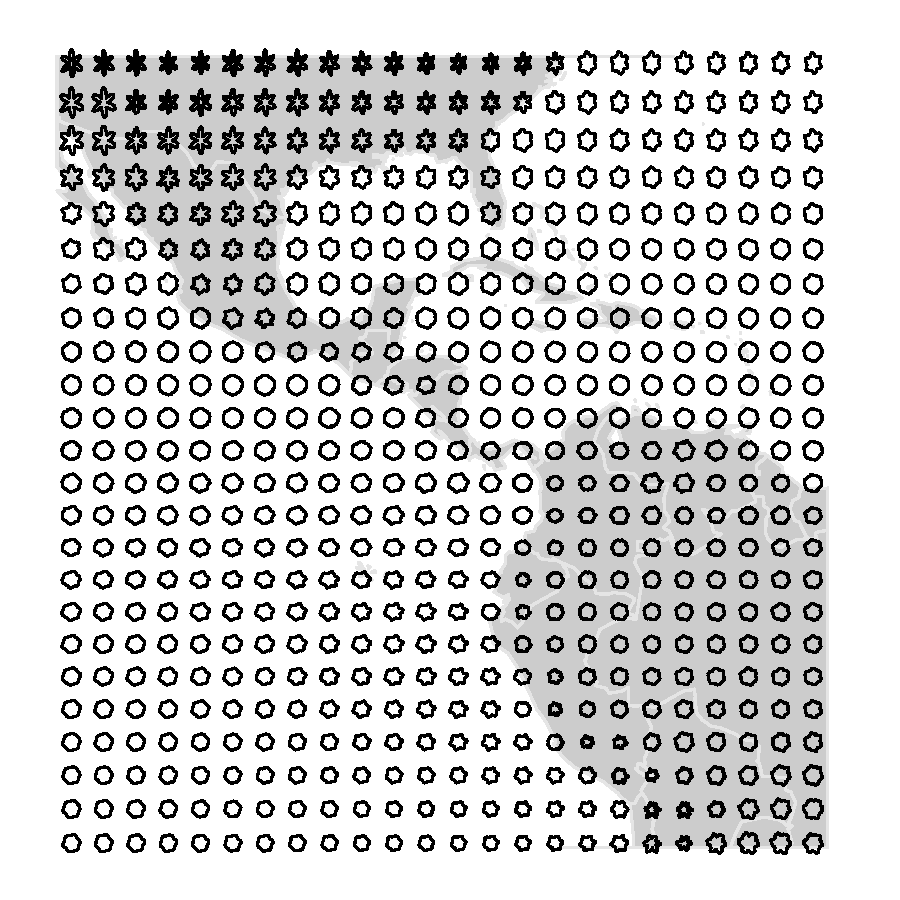
\includegraphics[width=3.5in]{nasa-glyph-all.pdf}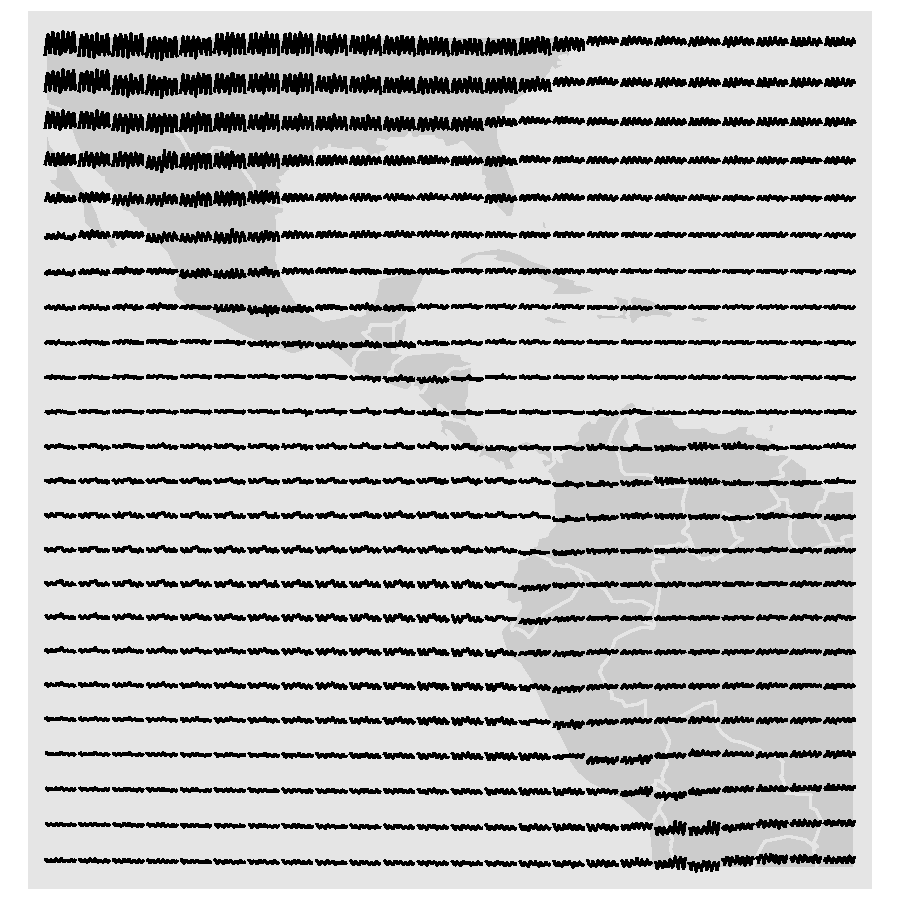
\includegraphics[width=3.5in]{nasa-glyph-ts-all.pdf}}
%\caption{Glyph-map of raw data, using star glyphs (left), and time series as glyphs (right).}
%\label{fig:glyph-map}
%\end{figure*}

Figure \ref{fig:gistemp-pred} shows the star glyphs for each spatial location of raw temperature for 1880-2011 across the USA. The major feature to notice is the pattern of missing values, icons that do not complete the full circle. The high noon position of the circle is the first time point, Jan 1880, and it is this early time period that has missing values are a lot of locations. It was for this reason that the temporal model was fit just to 1950-2010 data. Another important feature is variability, indicated by the thickness of the circle. Some locations, particularly in the north western mountain region, have big variability in temperature, both low minima, and high maxima. At these locaations there are large fluctuations from the long term mean.

\begin{figure}[htbp]
  \centering
  %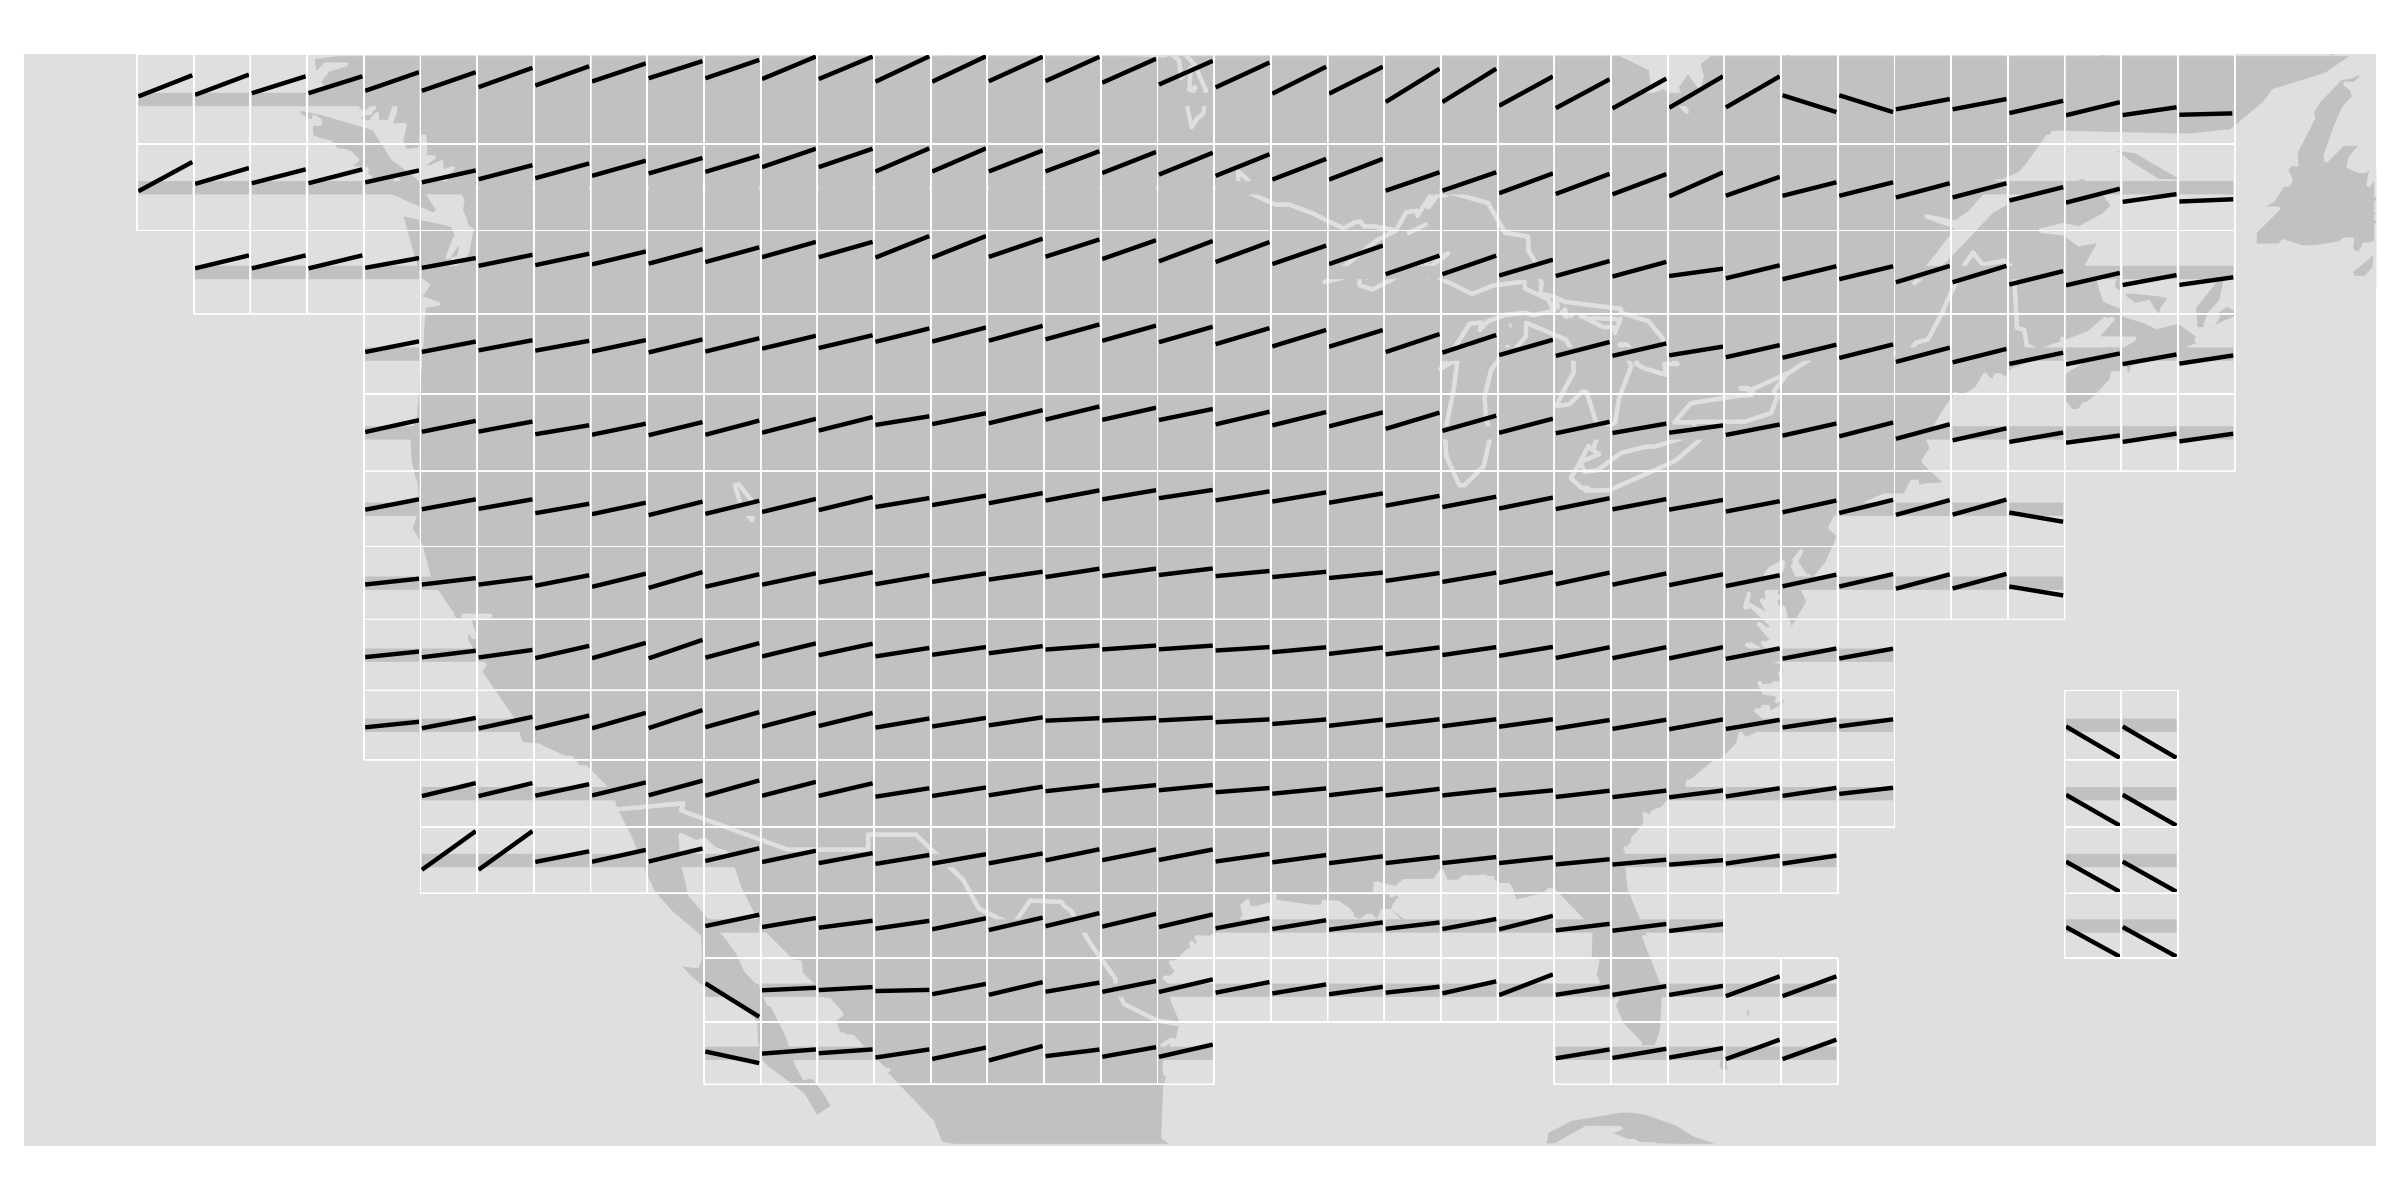
\includegraphics[width=1\linewidth]{gistemp-pred}%

  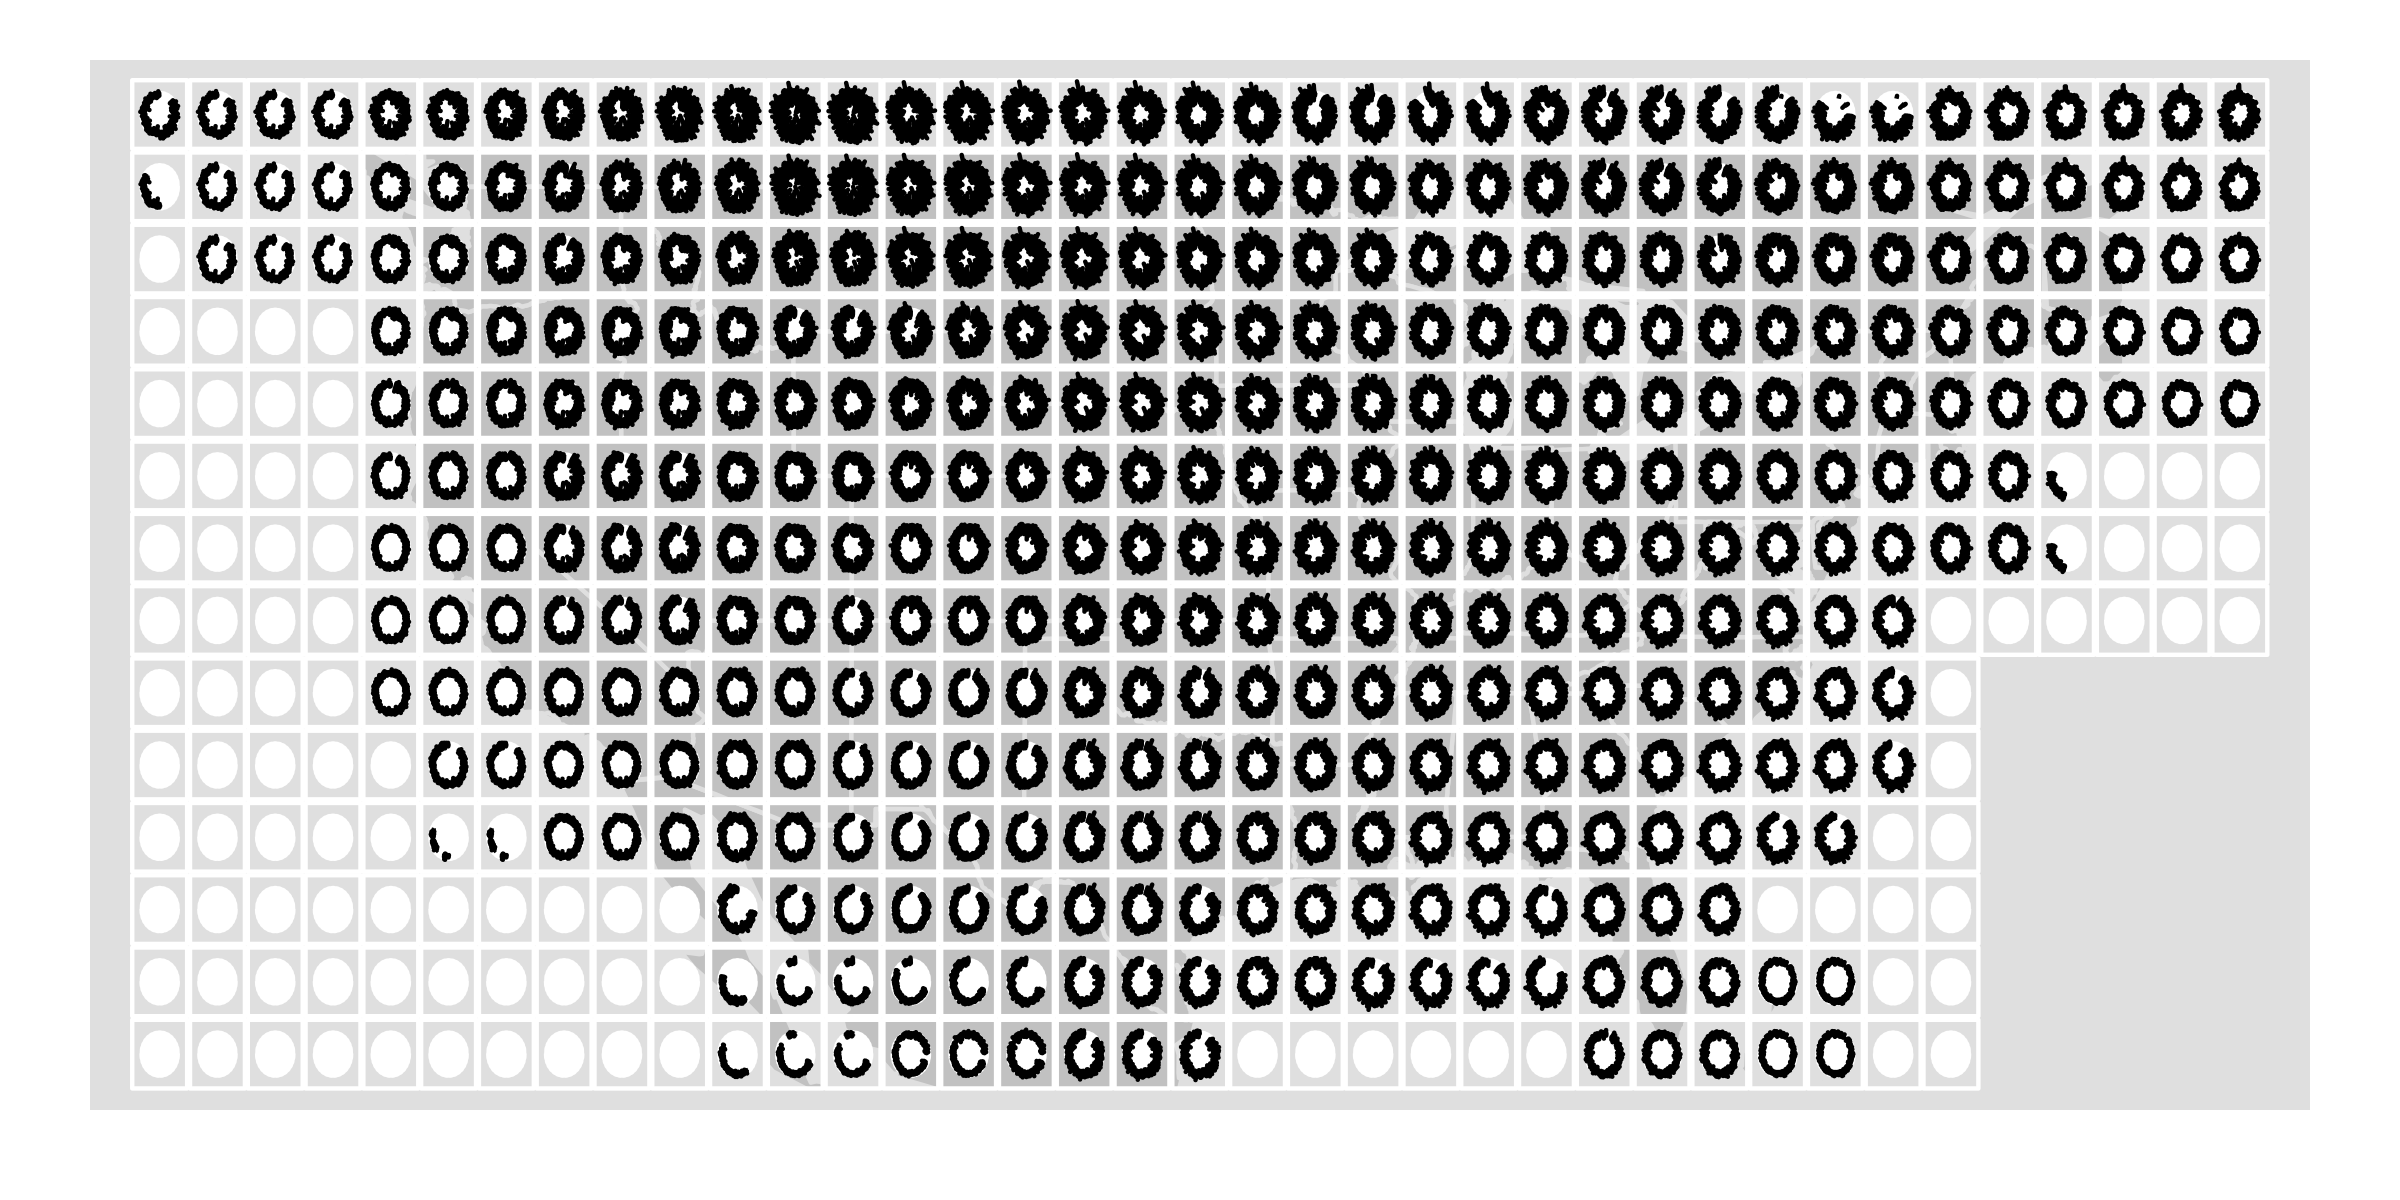
\includegraphics[width=1\linewidth]{gistemp-polar-raw}

  \caption{Glyph-map of raw temperature anomaly data, from 1880-2011. Gaps in the full circle indicate missing values, and thickness of the circle indicates more variability in the measurements.}
  \label{fig:gistemp-raw}
\end{figure}

*** Need to add reference circles.
 
Icons have been displayed on maps since the earliest displays weather forecasts, in the 1800s. In recent times, \citet{pickett:1988} introduced the idea of using icons on maps to display multivariate spatial data. This area of work has morphed into the field of metaphorical data displays, which creates abstract landscapes of spatial data, a digression from glyph-maps. \citet{gribov:2006} describes the use of glyph-maps for multivariate data also, with emphasis on the graphics software Gauguin. 


%\subsection{Glyph plots}

%Simple, but effective, technique that combines aspects of glyphs, facetted plots and map-charts. Particularly well suited for the type of temporal-spatial data, commonly seen in climate.

%Glyph-maps have attributes of both glyphs (stars, faces, profiles, ...), inviting exploration at the global level, and small-multiple time series, allowing local exploration of individual series. Allow to see both geographic context and individual locations simultaneously.

%Avoids one problem that plagues glyph displays: the ordering of the variables. Although some techniques exist to ameliorate this problem \citep{kleiner:1981,hurley:2010}, they are not necessary with time data because it is intrinsically ordered.

%These displays tend to be particularly effective when printed in large format, as the much higher resolution of print (600 dpi) compared to computer  screen (72-120 dpi) allows for much finer reading. These are high-density data displays in the best tradition of Tufte. Wall size maps are not usually practical during analysis, but are very engaging.

%Will first explore for regularly gridded data, a simple starting point and a common output of climate models, and then show a few simple extensions to deal with non-rectangular grids and irregular locations, as exemplified by raw climate data which is typically collect at irregular locations.

\section{Computation}~\label{sec:construction}

%A big advantage of glyph-maps is that they can be generated with existing graphics software after performing a simple pre-processing step, making them easily accessible to a wide audience. 
Creating a glyph-map, involves recognizing that they combine two structural components of the data: spatial location and data values. The spatial location is the major positioning component, and the data values are minor adjustments to these positions. For spatiotemporal data, the major axes are latitude ($y_{\amaj}$) and longitude ($x_{\amaj}$), and the minor axes are time ($x_{\amin}$) and some measurement ($y_{\amin}$), for example, temperature, or predicted temperature. The minor axes are rescaled to have range $[0, 1]$, and further adjusted to fit into the resolution of the spatial coordinates. The final values to be plotted are a simple linear combination, as given by 

\begin{equation}
\begin{array}{lll}
x_\text{ coordinate}&=& x_{\amaj} + w \cdot x_{\amin}\\
y_\text{ coordinate}&=& y_{\amaj} + h \cdot y_{\amin}, 
\end{array}\label{coords.eqn}
\end{equation}
where $w$ and $h$ are width and height respectively. The width and height will typically take into account the resolution of the major axes, that is, the minimum difference between consecutive locations.

Computing the coordinates for star glyphs is achieved by using polar coordinates,  $r=y_{\amin}$, and $\theta=x_{\amin}$, both scaled to be between 0 and 1. Then the glyph coordinates are given by 
\begin{equation}
\begin{array}{lll}
x_\text{ coordinate}&=& x_{\amaj} + \frac{w \cdot r}{2} \sin(2 \pi \theta) \\
y_\text{ coordinate}&=& y_{\amaj} + \frac{h \cdot r}{2} \cos(2 \pi \theta).
\end{array}\label{coords.polar.eqn}
\end{equation}
Note that, this is is a non-standard conversion to polar coordinates, but this conversion provides a time line that starts at 12 o'clock and wraps around the origin in a clockwise fashion.

Figure~\ref{fig:cycle} shows average monthly temperature as time (Cartesian coordinates) and star (polar coordinates) glyphs, for a subset of the spatial region. In this case, the star glyphs are not as effective as the linear glyphs: perhaps because of the absence of cyclical pattern.

*** Perhaps replace these figures with something from the GISTEMP data.

\begin{figure}[htbp]
  \centering
  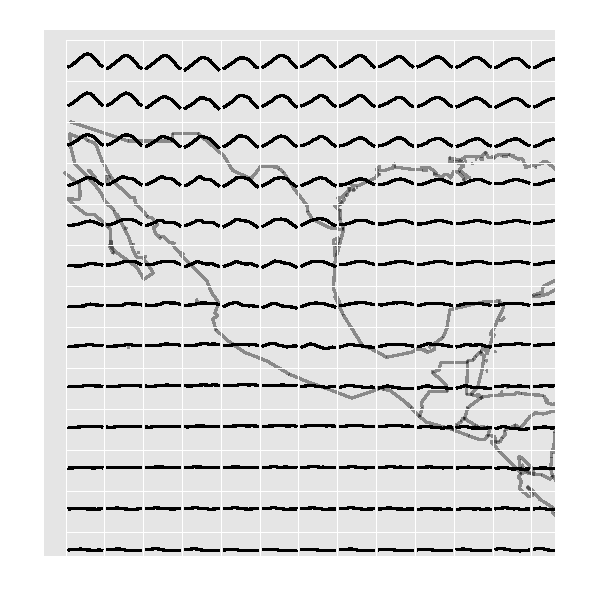
\includegraphics[width=3in]{month-cartesian}
  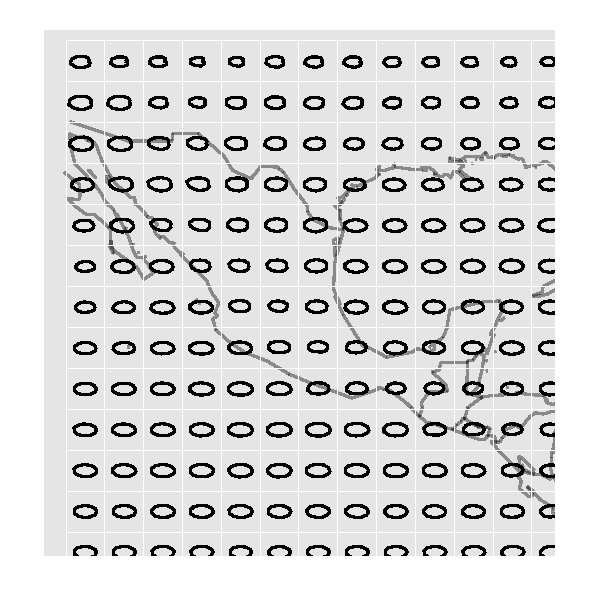
\includegraphics[width=3in]{month-polar}
    
  \caption{Monthly averages in (left) Cartesian coordinates and (right) polar coordinates.}
  
  \label{fig:cycle}
\end{figure}


Figure \ref{fig:templates} gives some small examples of time series with prototypical trends, shown both in cartesian coordinates and polar coordinates. Differences between linear and nonlinear trend are more apparent in the time series icons, and are effectively lost in polar coordinates. The star plots are most effective in exposing cyclical patterns due to seasonality. Seasonality appears like floral cartoons in the polar coordinates, with peaks forming petals. What might be surprising is that time series that seem to have opposing trends in cartesian coordinates don't necessarily show this symmetry in polar coordinates. The area of glyphs in polar coordinates mainly reflect the average value of a time series, while its shape shows deviations from average values. 

Since the coordinates are linear combinations of two variables, it is possible to build these these time series icon displays interactively, illustrated by software packages that have incorporated tours \citep{cook:2006}, such as DataViewer \citep{buja:1986}, XGobi \citep{swayne:1991} or GGobi \citep{swayne:2003}.  This technique is used to good effect in \citet{buja:1996a}, and was used to examine the climate data in \citet{hobbs:2010}.

% Show the glyph-map for de-seasonalized data, and describe what we
% see differently from the facetted map

%\begin{figure}[htbp]
%  \centering
%  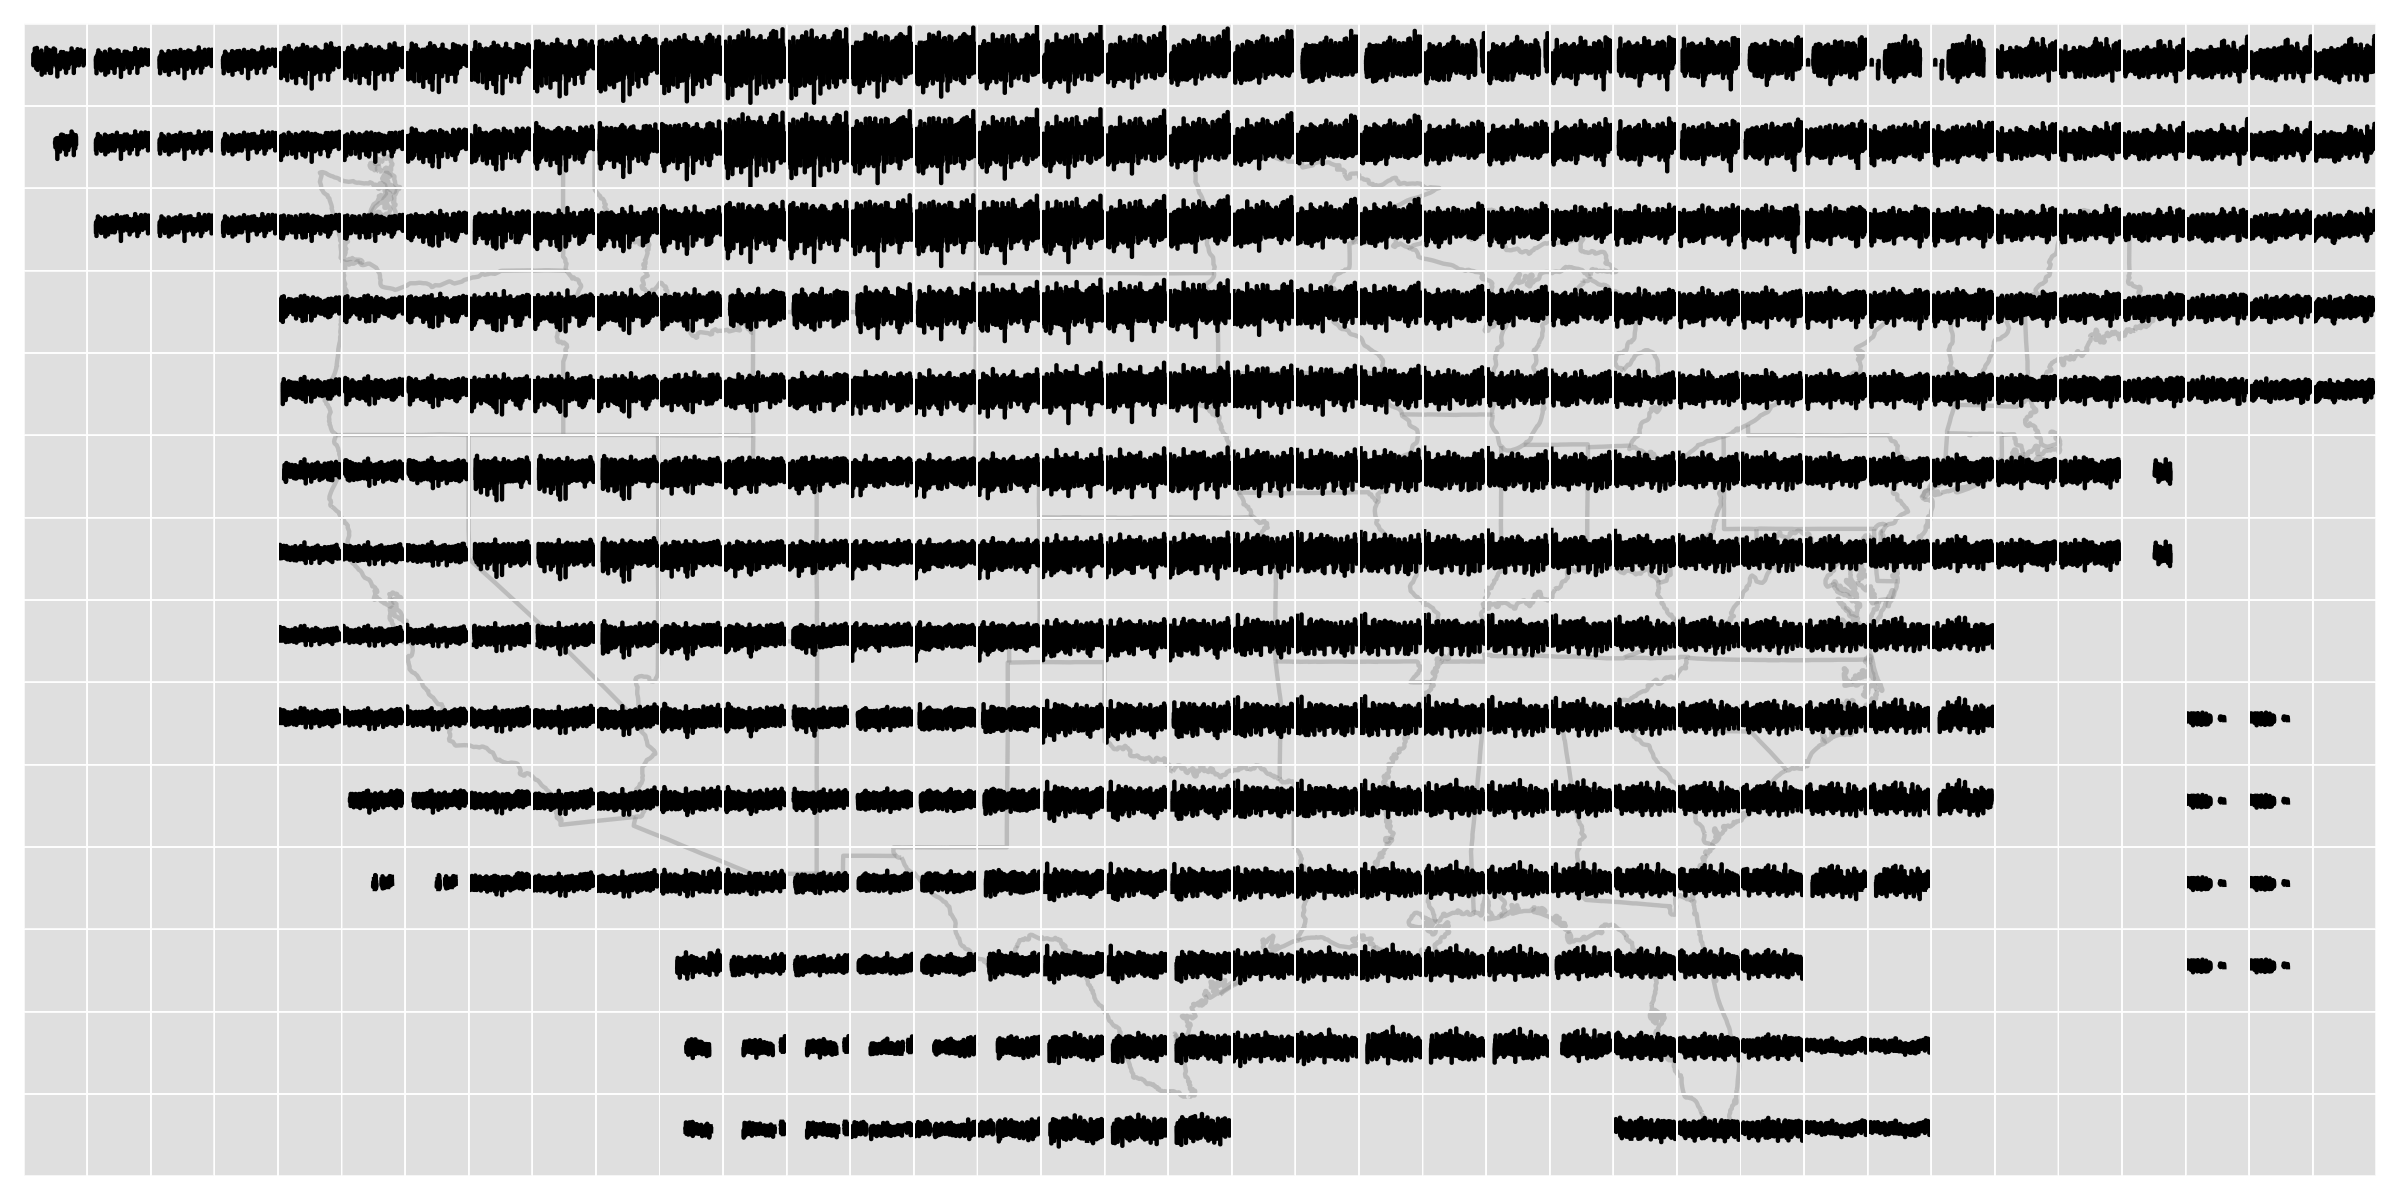
\includegraphics[width=1\linewidth]{gistemp-raw}%

%  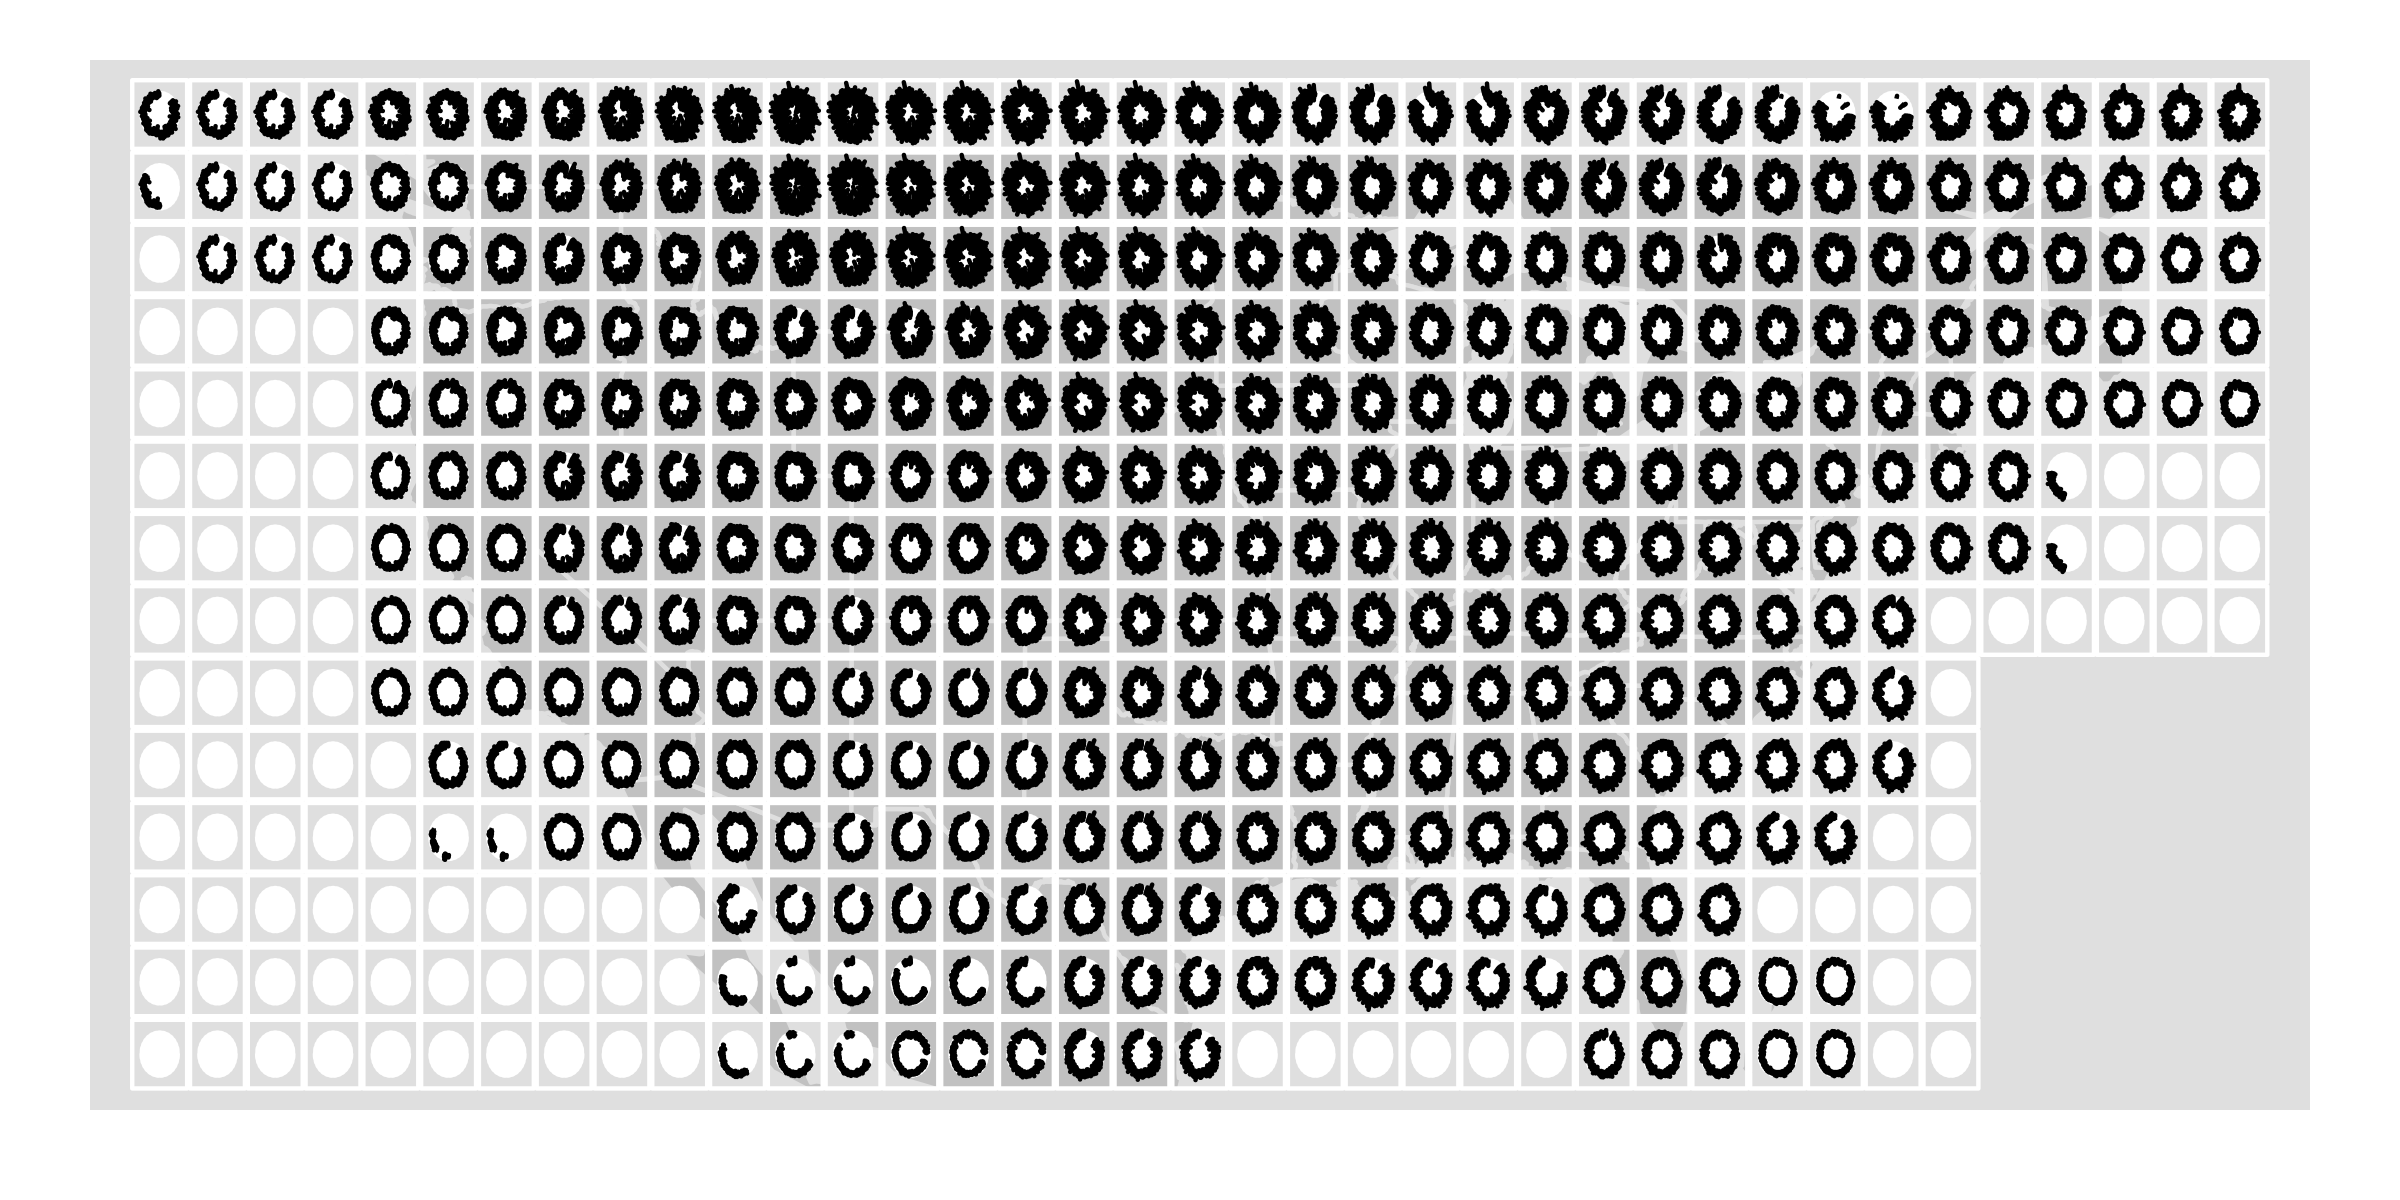
\includegraphics[width=1\linewidth]{gistemp-polar-raw}

%  \caption{Glyph-maps of gridded raw temperature anomaly data}
%  \label{fig:ref-gistemp}
%\end{figure}



\section{Reference frames}~\label{sec:reference}

A \emph{visual reference grid} \citep{cleveland:1993a} is fundamental
to a good data visualization, in order to compare values mapped to
position along a line. For glyph-maps, it is not feasible to make a
full set of axes for each icon, because these would dominate the
picture. Visual reference grids need to be post-attentive
\citep{healey}, de-emphasized, and serve as posterior look up after
the patterns in the data have been read. For glyph-maps, we need to be
able to make the following types of comparisons across icons:

\begin{itemize} \itemsep 0in
\item Slope, or trend
\item Intercept, or average value
\item Variance, or size
\end{itemize}

The structured spatial arrangement of icons in a glyph-map helps to compare the patterns of shape, like slope, intercept, or size, across icons. But, additional clues would make it comparisons easier. For example glyph-map in Figure~\ref{fig:gistemp-pred}, contains two additional guides, a reference grid, and reference line. Both are drawn in white, because it is minimally perceptible (post-attentive), relative to the dark black ink of the data.

The reference grid is a box, framing each icon, representing the spatial grid. It helps to read differences in slope and intercept. Slope is read by comparing the left and right endpoints of the predictions (line) against the relative location on the frame. Intercept is compared by reading the ``average'' position of the line in the box, near the top, or near the bottom. The reference line, drawn as a horizontal line at the average predicted temperature value, provides for better reading of the intercept. The average value for the temperature anomaly data is not the same across the map: at higher latitudes the temperatures are uniformly higher, but at lower latitudes they are uniformly lower. (**** Can this be right? Would it mean that at these locations the temperatures 1950-2010 are much higher than the reference year temperatures?)

%Figure~\ref{fig:ref-basic} shows two reference grid variants: a line drawn at the overall mid-range, and a box drawn around each grid cell. We prefer using white for these references because it is minimally perceptible: you can see the grid easily when looking for it, but it does not otherwise distract from the perception of the graphic \citep{carr:1994}. When we add a reference to each location, as in Figure~\ref{fig:ref-basic}, we see not only a difference in shape between Northern and Southern hemispheres, but also average value. Without reference lines, it is difficult to see that average seasonal coefficients are much higher in the North than in the South.

% Think we might need to show the original figures of data with reference lines

*** Re-do these figures with zooms in on the GISTEMP data

\begin{figure}[htbp]
  \centering
  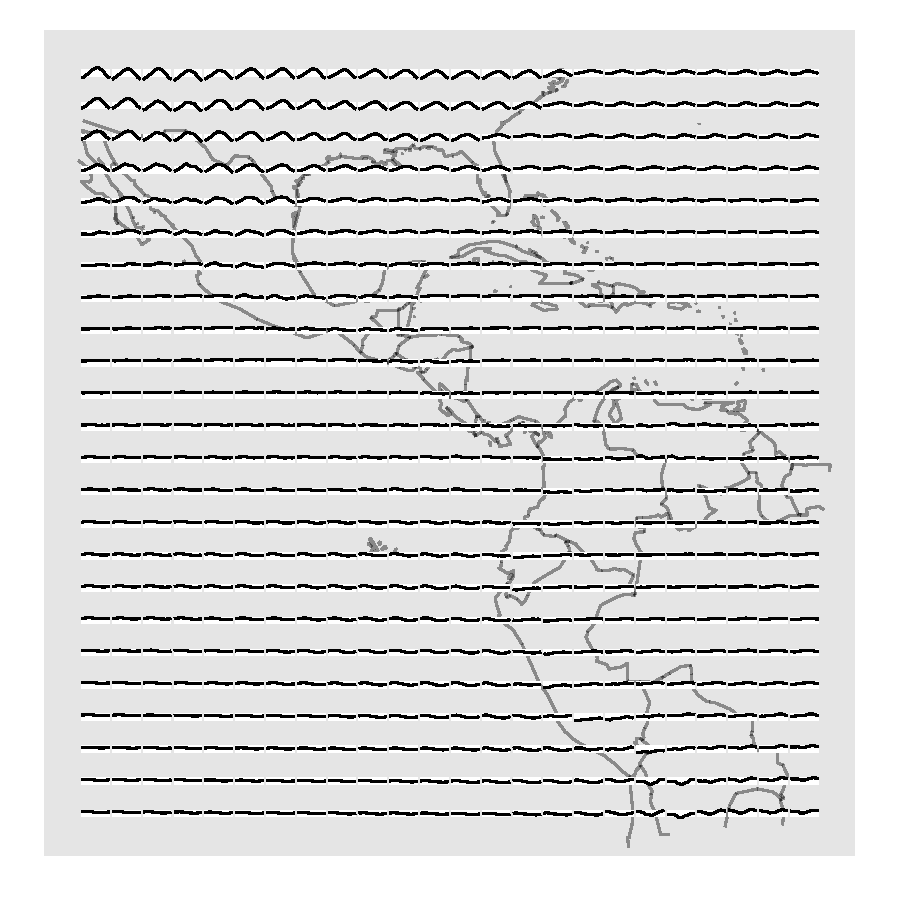
\includegraphics[width=0.5\linewidth]{ref-line}%
  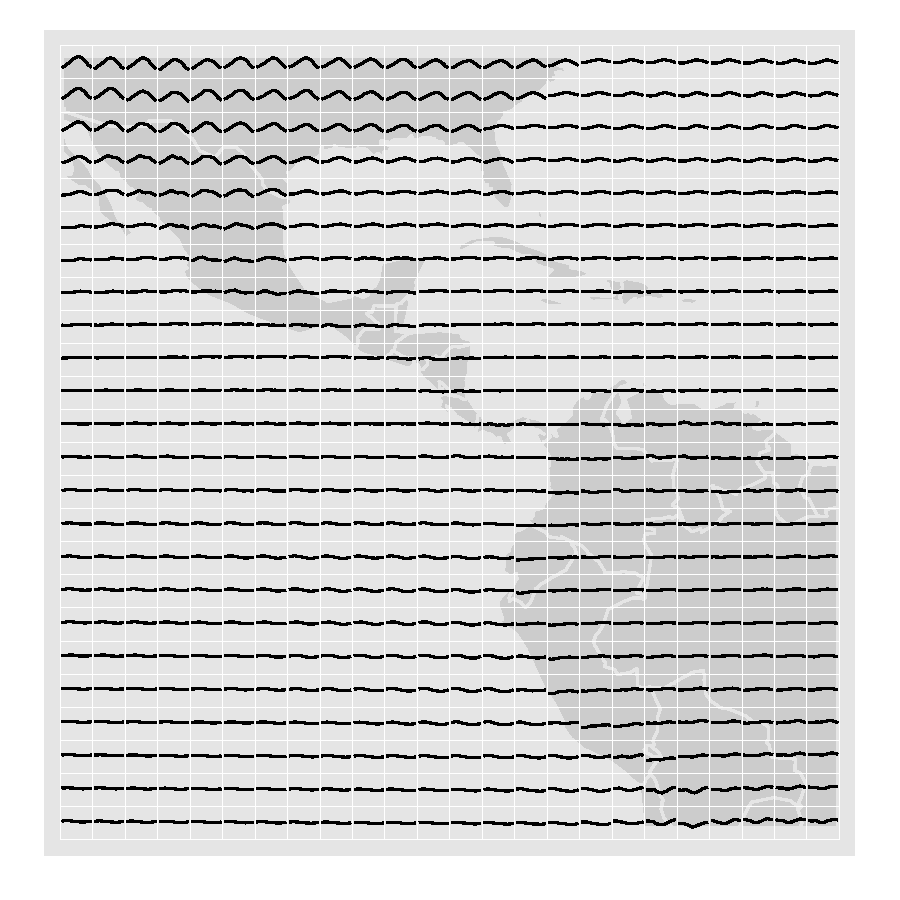
\includegraphics[width=0.5\linewidth]{ref-box}

  \caption{Glyph-maps of seasonal temperature patterns. Adding reference lines, (left) mid-range lines and (right) grid-cell boxes, makes it easier to see differences in glyph position, not just shape.}
  \label{fig:ref-basic}
\end{figure}

For star glyphs, the reference frames are also useful, but the reference line would be replaced by a reference circle, drawn at the average data value. Figures \ref{fig:templates} and \ref{fig:gistemp-raw} show examples.

%*** Re-visit this next paragraph - its a little too airy-fairy, and the plot with color needs to have the color dampened more. Its way too dominant. This paragraph is too speculative for the paper, so removing it from first draft.

%It's also often useful to display other types of reference information. You are only limited by your imagination (and the capabilities of your graphics software), but two simple ideas are to (1) vary the colour or transparency of glyphs or references, or (2) use an additional layer to highlight special points. Figure~\ref{fig:ref-adv} illustrates these ideas to display the month with the highest temperature at each locations. Careful colour choice is necessary so that this information is perceptible, but not distracting.

%\begin{figure}[htbp]
%  \centering
%  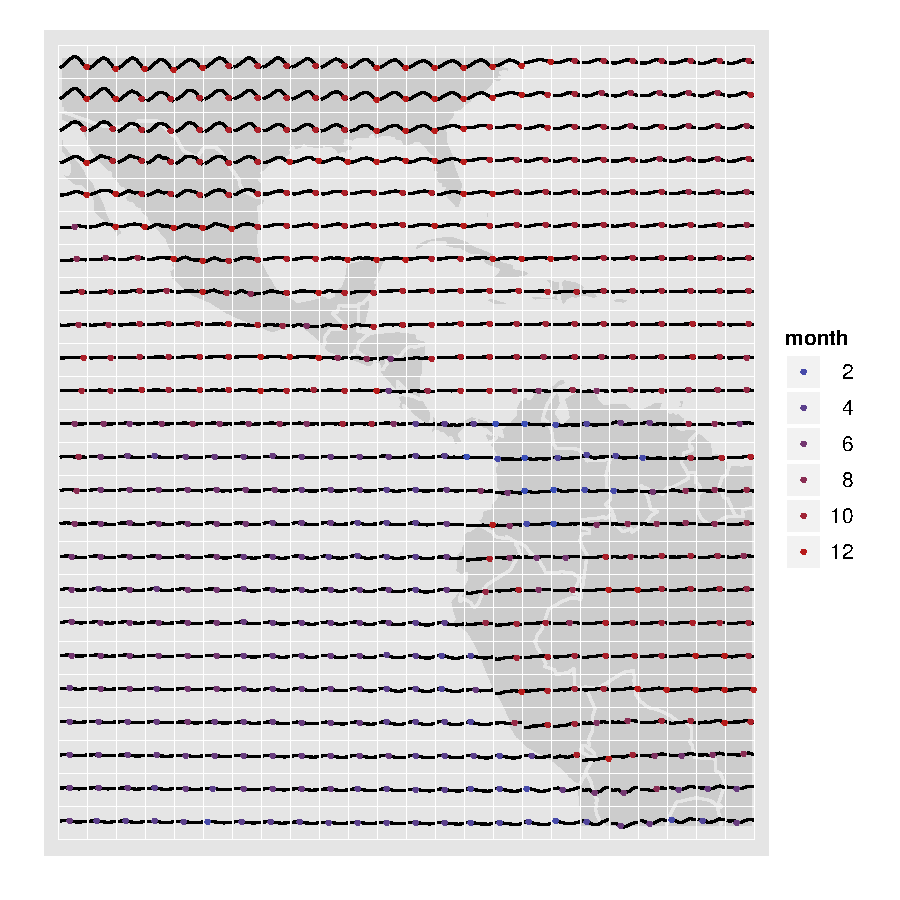
\includegraphics[width=0.5\linewidth]{ref-max-1}%
%  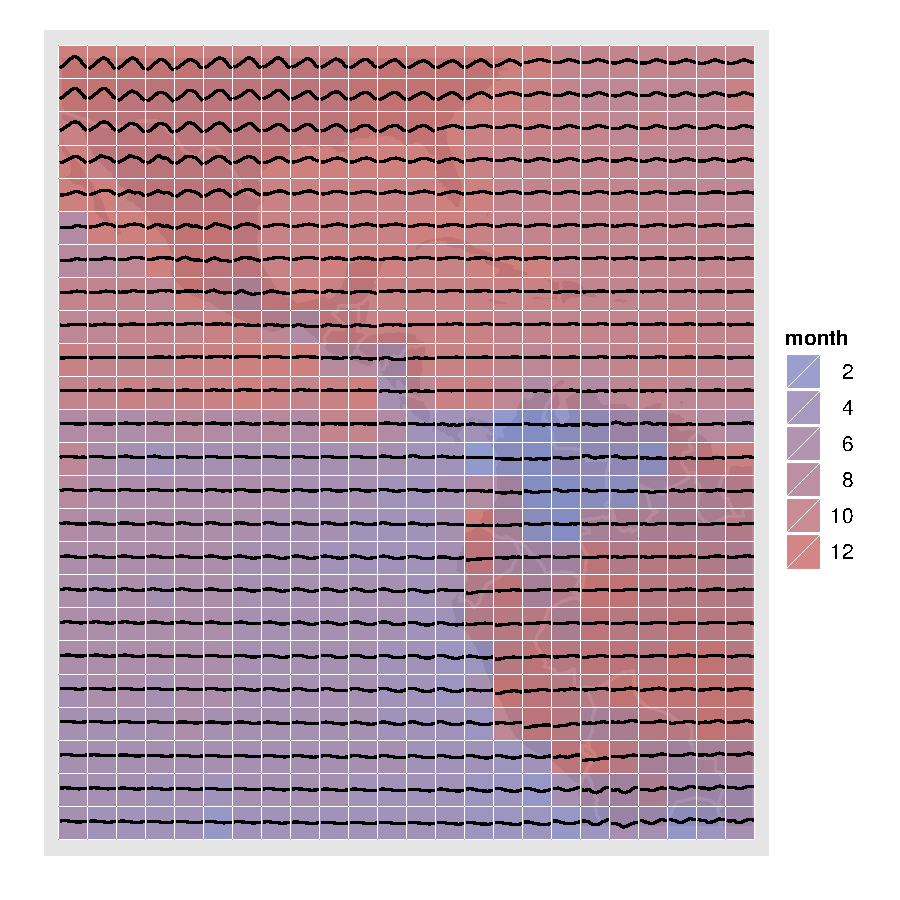
\includegraphics[width=0.5\linewidth]{ref-max-2}
%  \caption{Glyph-maps of seasonal temperature patterns also showing the month with the highest temperature using (left) an additional layer of points and (right) changing the background colour of the reference grid.}
%  \label{fig:ref-adv}
%\end{figure}

%A particularly useful summary when to add when displaying model predictions, is some measure of model fit. This makes it easier to avoid over-interpreting predictions from poorly-fitting models.


%*** Adding a circular reference line helps to pick out these deviations.

\section{Perception of structure}~\label{sec:scale}

Glyph-maps using trend lines enable the reading of trends across spatial locations directly from the plot. In comparison, to read trend from facetted colored maps one needs to spot the difference between the different maps.  Compare the facetted map in Figure \ref{fig:facetted-map} with the glyph-map of de-seasonalized data in Figure \ref{fig:nasa-deseas-glyph}. The glyph-map provides a texturing over the map. The El Ni\~no event is still the primary visble structure, the region that has a bump in the middle of the time series, correspondingto the hot 1997-1998 period. We can also see other temporal features: that the temperatures are generally more varied over land, there are a few locations with dramatically increasing temperature in the later years typically in locations that are the high elevation areas, along the Andes, and Sierra Madre Occiddental in Mexico.

The glyph-map can be considered to be small multiples as named by \citet{tufte:2001}, in this case, small multiples of time series. By laying the time series out on the spatial grid, the main task expected of the viewer is comparing the temporal patterns from one location to the next. In contrast, in the small multiples used in the facetted colored map, the viewer is expected to compare the patterns in the maps from one year to the next, for corresponding months. (See \citet{carr:1999} for a discussion on perceptual grouping.) That is, compare and contrast maps with factted colred map, or compare and contrast time series using the glyph-map. One draw-back of the glyph-maps, particularly if linear trend is displayed as an icon, is they may suffer from the Z\"ollner Illusion \citep{Zollner} which is visible in Figure \ref{fig:gistemp-pred}. On the other hand, comparing images require that we play a spot the difference game, which is perceptually difficult \citet{busey}.

An alternative, to both of these approaches, to focus attention on specific parts of the data calculate the relevant statistic for each location and display these values as color on a map. For example, to study the warming or cooling trends, we might calculate the slope of a linear model at each location and color tiles across the map by the value of the slope. From this we might see the increasing temperatures at higher altitudes in the NASA temperature data. However, we would fail to see the finer points of the time series, that the increase is not as simple as a linear increase. In addition, Cleveland's \citep{cleveland:1993a} perceptual tests suggest that the reader can perceive the positional difference of the lines better than the color differences. Accurate perception of color differences is difficult.

\begin{figure*}[htp]
\centerline{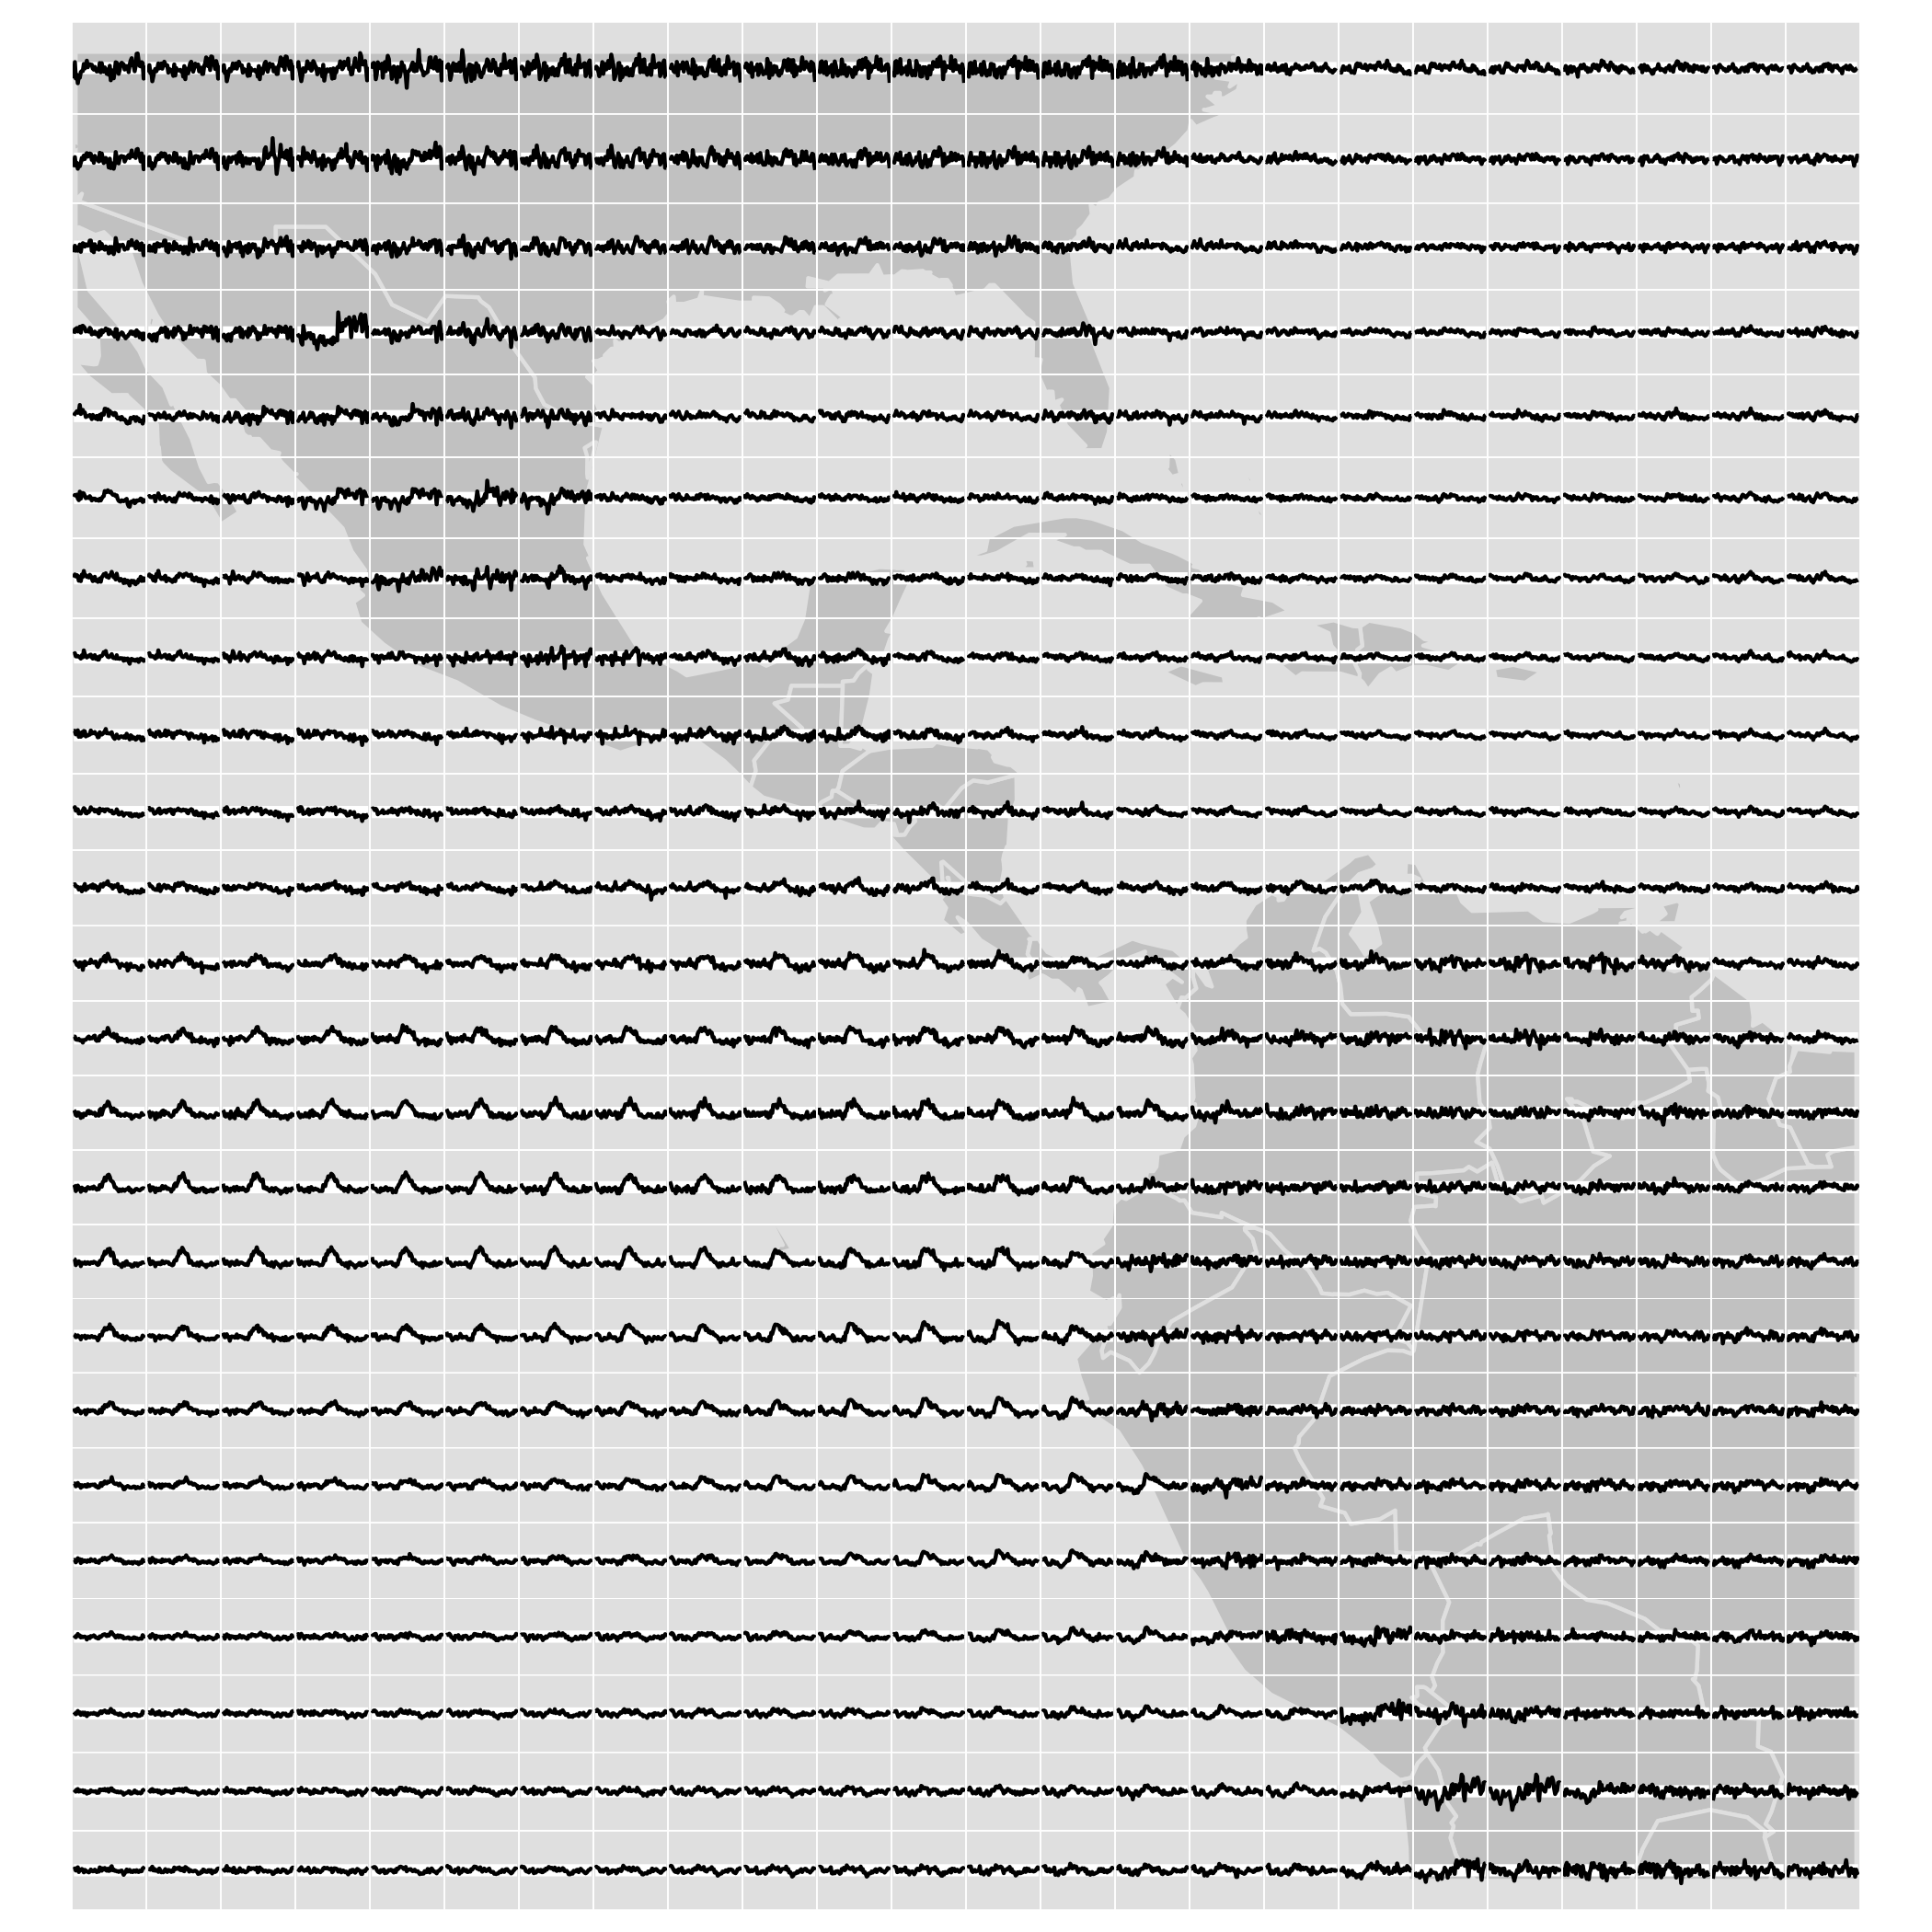
\includegraphics[width=4in]{nasa-deseas-glyph.png}}
\caption{Glyph-map of de-seasonalized temperature, to compare with Figure \ref{fig:facetted-map}. }
\label{fig:nasa-deseas-glyph}
\end{figure*}


\section{Effect of scale}~\label{sec:scale}

%*** Global/local min/max, remove intercept/average, data vs model scale
%*** This section needs to have plots re-done, once we have decided on the key pieces

Scaling of the data, into the values used for each glyph, emphasizes different aspects of the data. For spatiotemporal data the most natural scale is to use the global minumum and maximum, because the temporal variables are measuring the same information, and we want to make comparisons across the spatial region. The icons will have size relative to the magnitude of the full range of the data. Locations with overall large temperature will catch the focus. Figure \ref{fig:nasa-deseas-glyph} shows data scaled to 0 to 1 based on the global minimum and maximum, using:

\begin{equation}
y_{st} = \frac{y_{st}-y_{min}}{y_{max}-y_{min}} %\times 2 - 1
\label{scale1}
\end{equation}

\noindent where $y$ is the variable used on the minor axis in equations \ref{coords.eqn}, \ref{coords.polar.eqn}, $y_{min} = \mbox{minimum}\{y_{st}; s=1, \dots S, t=1, ..., T \}, y_{max} = \mbox{maximum}\{y_{st}; s=1, \dots S, t=1, ..., T\}$, $S=$ is the number of spatial locations and $T=$ is the number of time points. In addition, $y_{st}$ may be further scaled by doubling and subtracting 1 to give values between -0.5 and 0.5 for using in equations \ref{coords.eqn}, \ref{coords.polar.eqn}.

Alternatively, scaling locally at each spatial location enables exploring shape differences, particularly seasonal patterns, from one location to another:

\begin{equation}
y_{st} = \frac{y_{st}-y_{s,min}}{y_{s,max}-y_{s,min}} %\times 2 - 1
\label{scale2}
\end{equation}

\noindent where $y_{s, min} = \mbox{minimum}\{y_{st}; t=1, ..., T \}, y_{s,max} = \mbox{maximum}\{y_{st}; t=1, ..., T\}$. With the local scaling, the shape of the icon, for example, differences in the seasonal patterns over spatial locations, are emphasized.  Fig \ref{fig:scaling} shows glyph-maps generated usng both global scaling (left) and local scaling (right) for the NASA temperature data. On the global scale, the El Ni\~no blip in temperature is primarily visible, along with the generally flat series over most water locations, and somewhat increasing or variable temerpatures over land. The local scale emhpasizes the individual shapes: The El Ni\~no pattern is visible, but extend to a larger spatial region including the Caribbean, dramatic linear increases across the Andes, decreases in the Gulf of Mexico. (The local scale is equivalent to using individual scales in the facetted graphics of \texttt{ggplot2}). One caution, with local scale, the viewer needs to realize that the scale is not relative, big patterns in some locations might be just tiny effects. To indicate this on the locally scaled data plots, using a very pale coloring to code the original scale in the tiles, might help puts patterns in perspective.

Other types of shifting and scaling can be useful. The mean and standard deviation might be used to standardize values, or the median and interquartile range, might be useful with some types of data. Shifting the values at each location to have mean zero, places more focus on the trend. This is particularly important for the star glyphs, where differences in the average value lead to unintuitive patterns in the resulting glyphs (eg Figure \ref{fig:cycle} star glyphs obscure the seasonal pattern).  In this situation we would use $y_{st}-\bar{y}_s$ instead of $y_{st}$ in equations \ref{scale1}, \ref{scale2}, with minima and maxima calculated on the mean-shifted data.

%Another way to think about these scale options is partitioning the data structure into shape, magnitude and shift components. The different ways to scale emphasize these different components. The shift component can be extracted from the data in different ways, using the intercept from a linear model, for example, instead of the average. 


%**** This is different - I think it just confuses the topic of scaling. Because the GAM is not used to rescale the data, you still have to do that using the local or global scling equations above. Moving the discussion to ``What to plot''. 

\begin{figure}[htbp]
  \centering
  %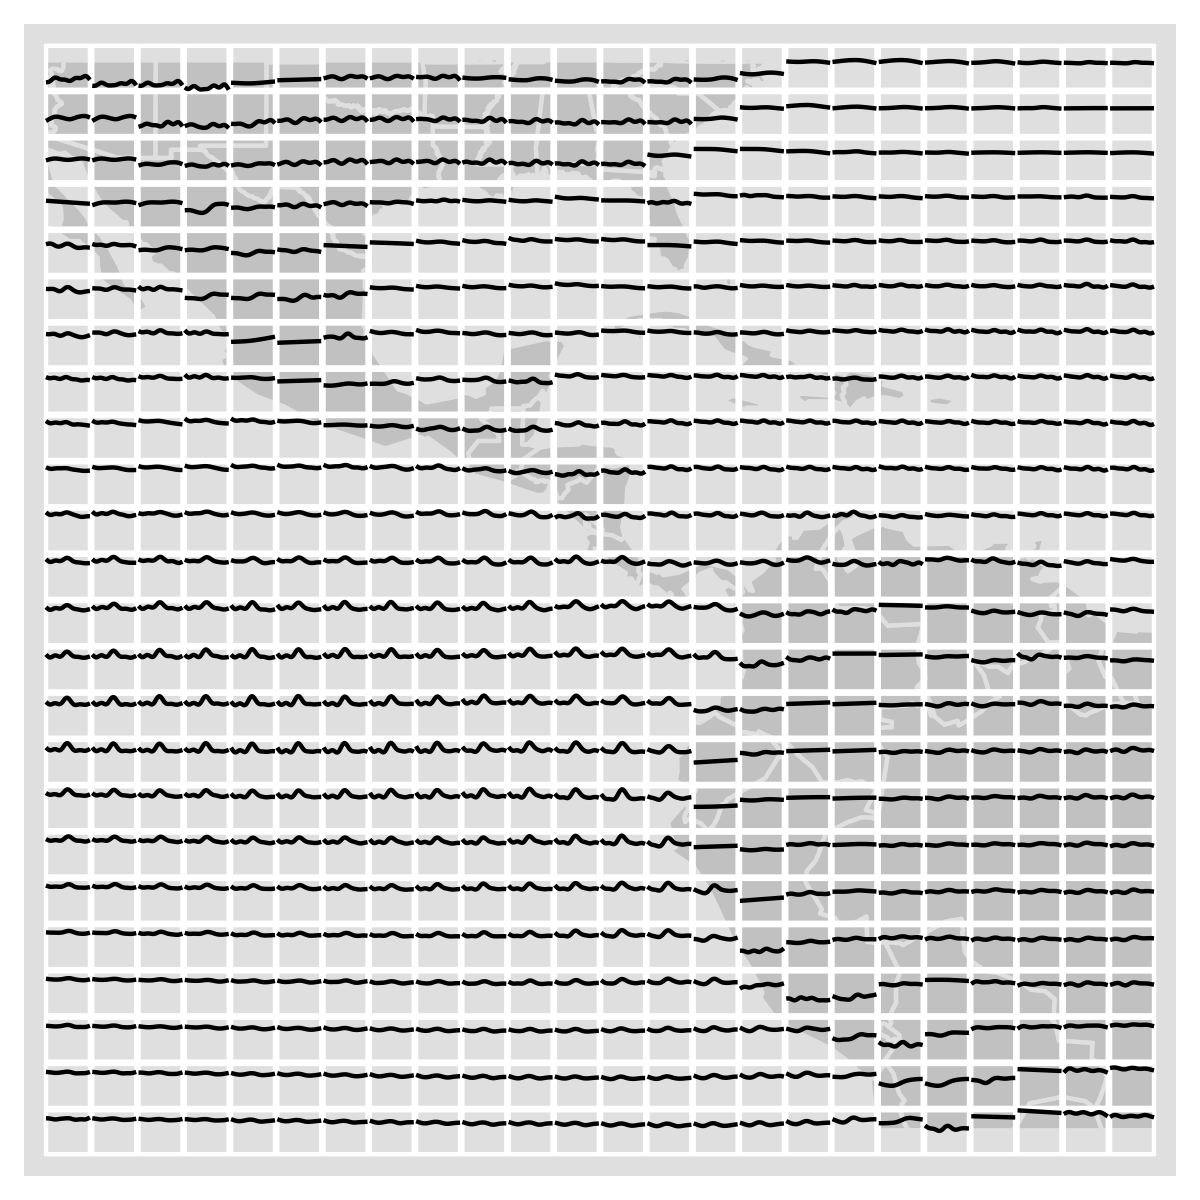
\includegraphics[width=0.33\linewidth]{month-rescale-none}%
  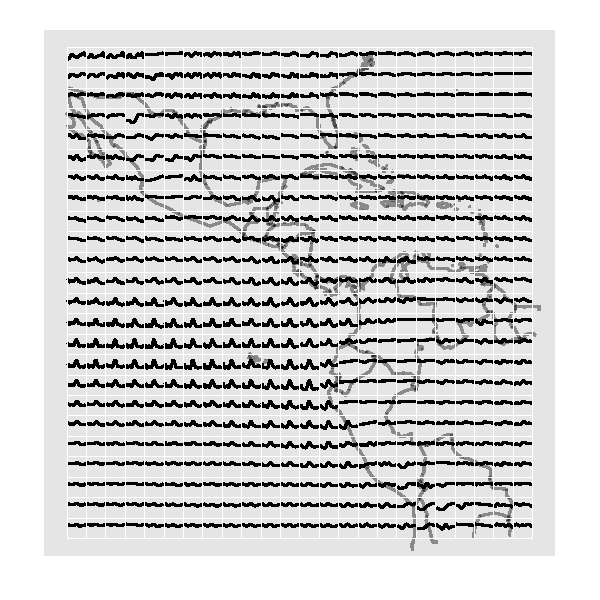
\includegraphics[width=0.5\linewidth]{month-rescale-max}%
  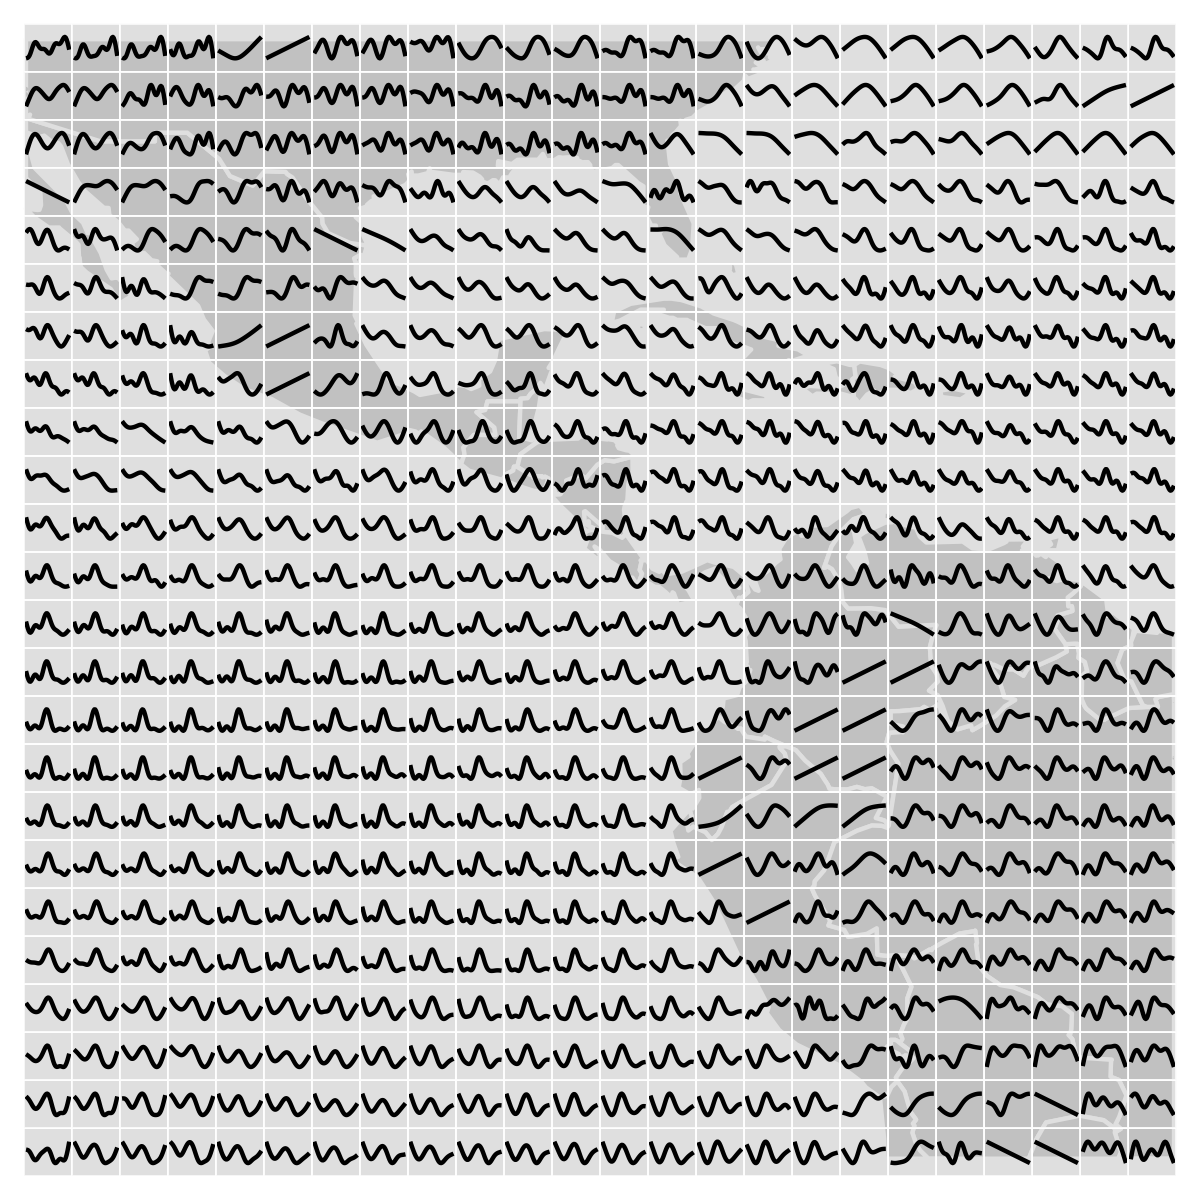
\includegraphics[width=0.5\linewidth]{month-rescale01}
  \caption{Smoothed de-seasonalized daily temperature glyph-map. (Left) %unscaled, (center) 
globally scaled, (right) locally scaled.}
  \label{fig:scaling}
\end{figure}

%A possible compromise is to use line colour to display the standardising variable, as shown in Figure~\ref{fig:scaling-col}.  This makes it possible to see the individual patterns while still retaining some ability to see which shapes represent small absolute changes.

%\begin{figure}[htbp]
%  \centering
%  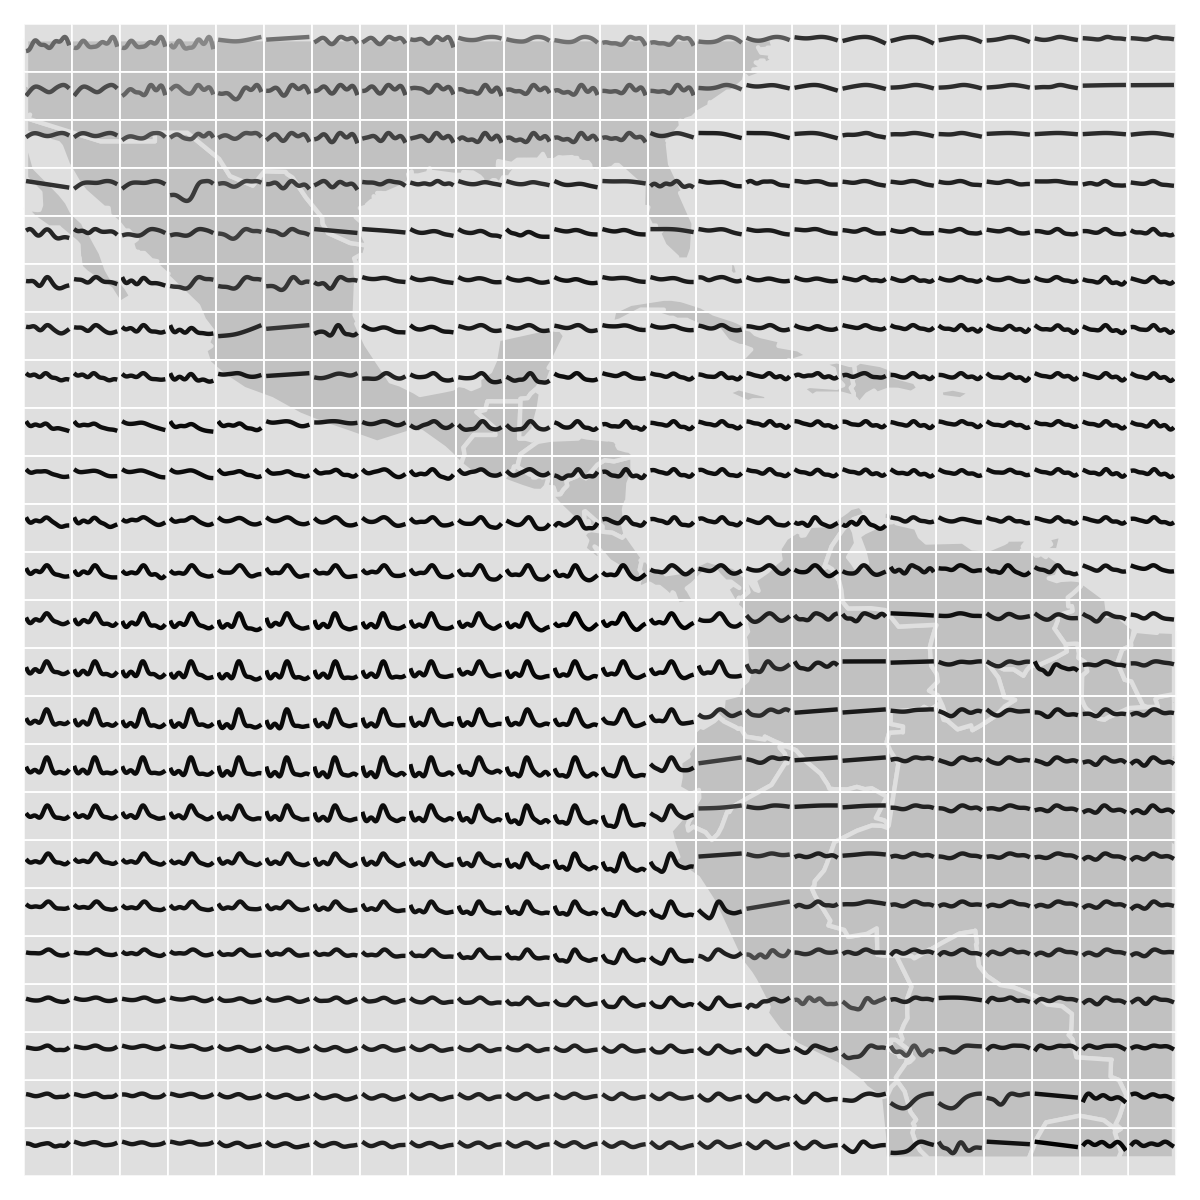
\includegraphics[width=0.33\linewidth]{month-rescale01-col}
%  \caption{Adding colour to scaled plots. Here each location has been scaled to range $[0, 1]$ and colour mapped to the range of the original predictions.}
%  \label{fig:scaling-col}
%\end{figure}

%Other types of scaling may be interesting to explore, such as a classical scaling using the mean and standard deviation.

%Equivalent to using individual scales in facetted graphics. 

One more important point: if a model summary is displayed in the glyph-map, such as the predicted values, it may be important to force the scale to that of the original data. Displaying the predicted values in the absence of the raw data scale can skew the interpretation of the magnitude of the effect. 

\section{What to plot: raw data, trend lines, residuals,  seasonal}

Structure in temporal data is composed of different parts: global trend, seasonality and error. Extracting each of these for visualization improves the focus on different aspects of the time series. A generalized additive model \citep{wood:2006} with a seasonal term and a long-term smooth term can be useful. This is revealing for smooth models of surface temperature, shown in Figure~\ref{fig:scaling}. Each location is modelled using a generalized additive model \citep{wood:2006} with a seasonal term and a long-term smooth term. The three plots in the figure show the long-term smooth term. %Because some locations are uniformly warmer than others, the impact of changes across time are diminished. In the center plot, each location is scaled by dividing out the maximum, and on the right, each location is scaled to range $[0, 1]$. These emphasize individual changes but lose the ability to make global comparisons, and need caution when interpreting - a small absolute change gets blown up into a large relative change.
 %The three plots in the figure show the long-term smooth term. Because some locations are uniformly warmer than others, the impact of changes across time are diminished.

% is a extremely useful technique: product plots, ANOVA, ...  For glyph plots, it's often useful to partition the glyphs into shape and scale components, decomposing the values into a product of maximum and scaled values.  In this section we explore how decomposing each series into scale and shape components can be useful.

*** Need three plots here: trend, seasonality and residuals, shall we do this with NASA ozone data or stick to temperature?

Issues of scale relative to modeling. Switching from the data to model summaries bringsnew scaling issues. Often the scale of the raw data is ignored when the model is plotted, one usually shows just the line showing the trend, in the range of the trend. This has the effect of exaggerating the signficance of the model. Scaling the trend lines rlative to the range of the data may be useful sometimes.

\section{Generalization}~\label{sec:scatter}

Glyph-maps are not limited to time series plots. They are readily generalized to use any other type of display as an icon. Figure~\ref{fig:cloud} shows scatterplots as icons: low-cloud level is displayed horizontally and high-cloud level vertically. The bivariate relationship between the two types of clouds is explored spatially, and it is clear that it is different across the region. The second plot displays a loess curve fit to the data instead of the individual points, sharpening the view of association: most locations have a negative or zero association.   In the Gauguin software \citep{gribov:2006} one alternative is an icon based on a histogram, small univariate distribution displays for each glyph. 

*** Need to use local scaling here.

\begin{figure}[htbp]
  \centering
  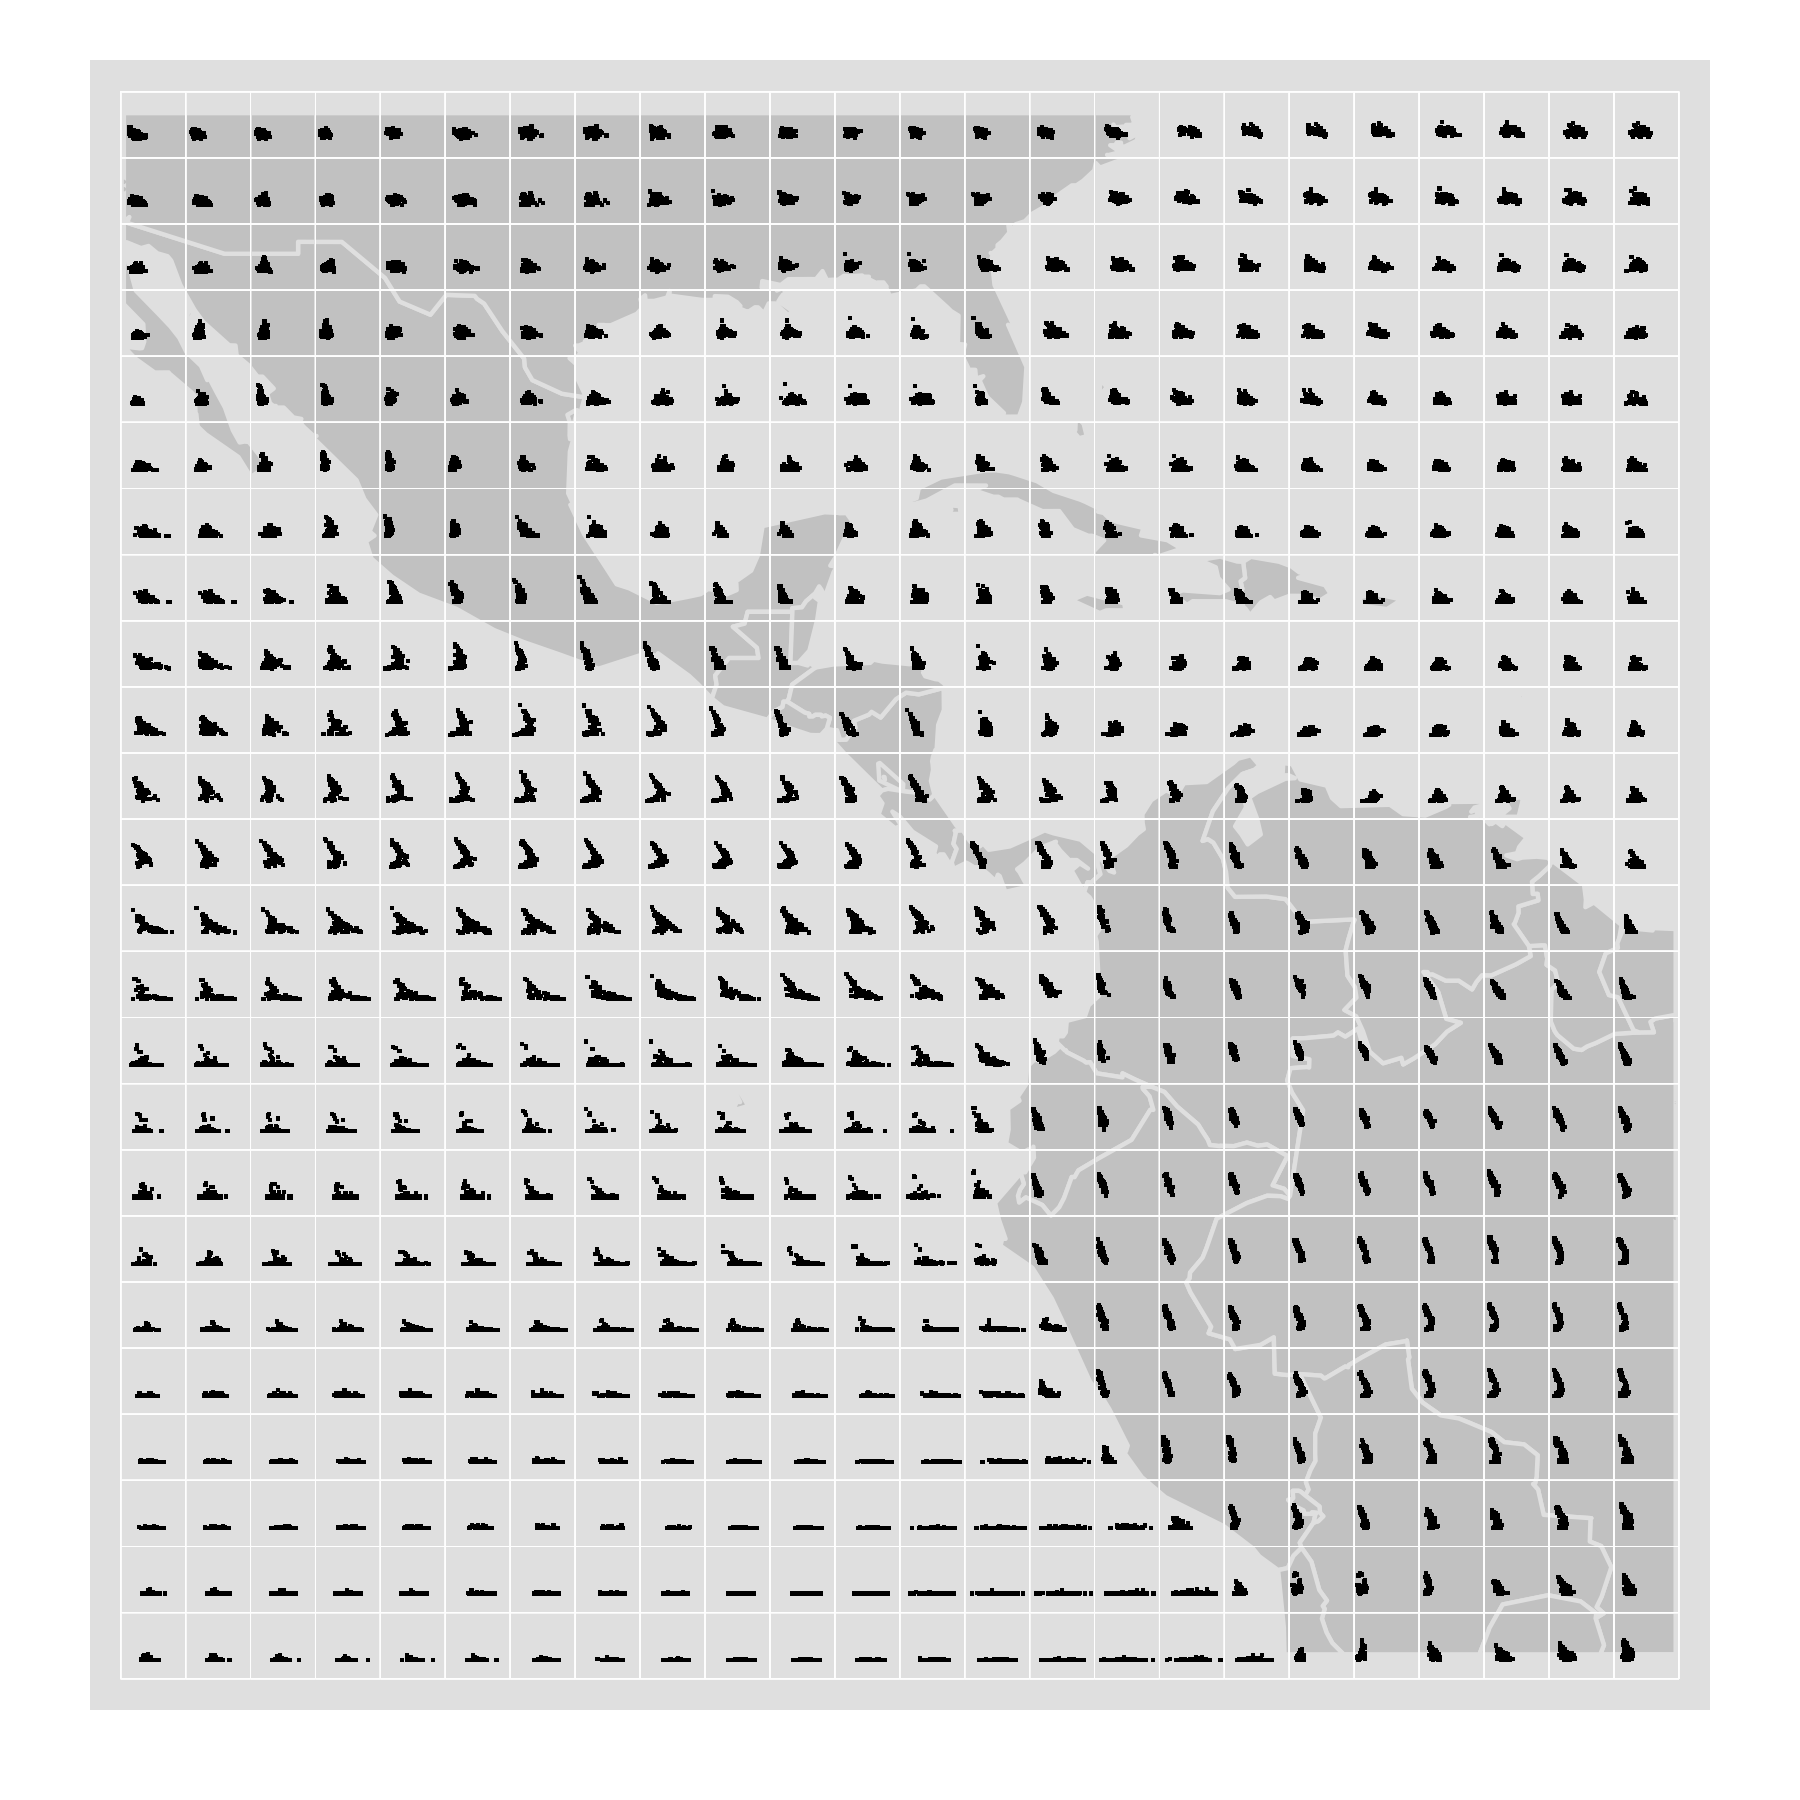
\includegraphics[width=0.5\linewidth]{clouds}%
  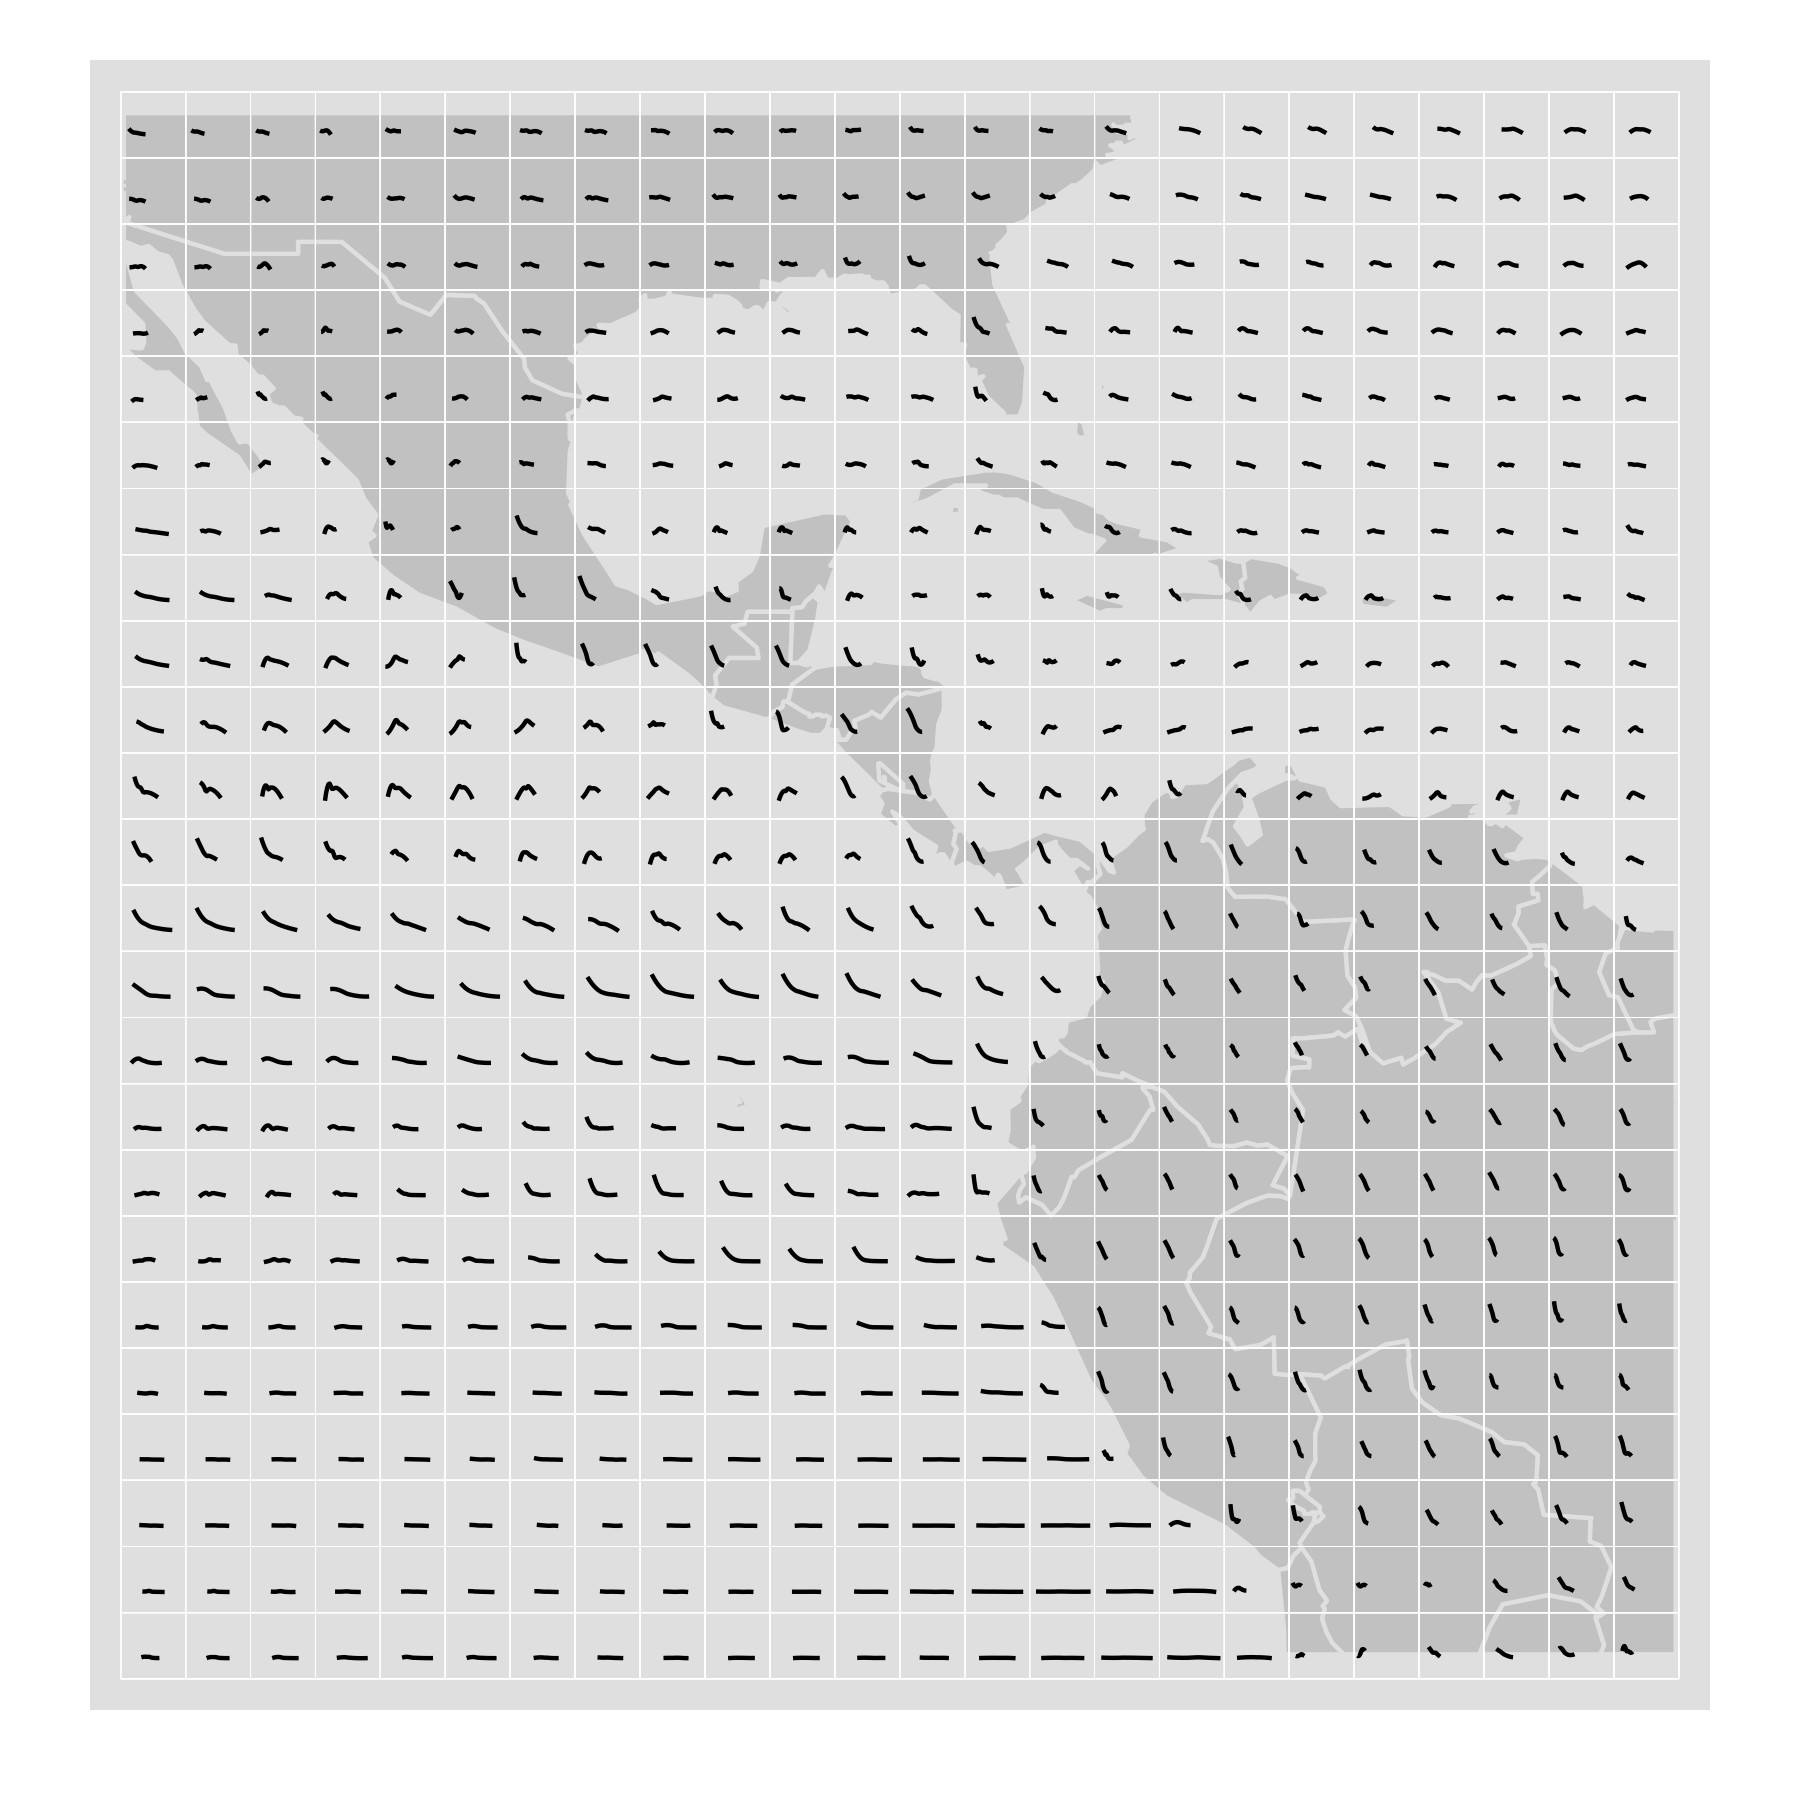
\includegraphics[width=0.5\linewidth]{clouds-smooth}

  \caption{Glyph-map showing (left) scatterplot of high-cloud vs. low-cloud and (right) smoothed (loess) curve fit to each location. The relationship between these two variables varies considerably over the spatial domain (particularly between land and ocean), but neighbouring locations tend to similar. }
  \label{fig:cloud}
\end{figure}

\section{Regular vs irregular locations}~\label{sec:irregular}

Regularly gridded spatial data helps with the perception of structure, because it helps to provide the reference frames upon which to make comparisons among the icons. When spatial locations are not on a regular grid, some difficulties arise. In this situation it is not clear what the scale of icons should be, there is no regular spacing. Some locations may be close to each other which would generate icons that overlap. 

\subsection{Non-rectangular grids}

Glyph-maps work best in mercator projection, where the icons are organized into rectangular microplots. Spatial coordinates are often not given in this coordinate system, and so may require a transformation into mercator projection coordinates.

\subsection{Irregular locations}
Figure \ref{fig:irregular} shows linear trends for monthly average surface temperature at stations in the USHCN (Version 2) ground station network.  It illustrates three challenges in working with irregular locations: there is no natural choice for icon size, icons can potentially overlap, and comparisons rely more heavily on the reference guides.  The icon sizes were chosen manually for these two plots, although the icons are displayed at about the same size, they correspond to 1 degrees and 0.5 degrees square respectively in the geographical coordinates. 
\begin{figure}[htbp]
  \centering
  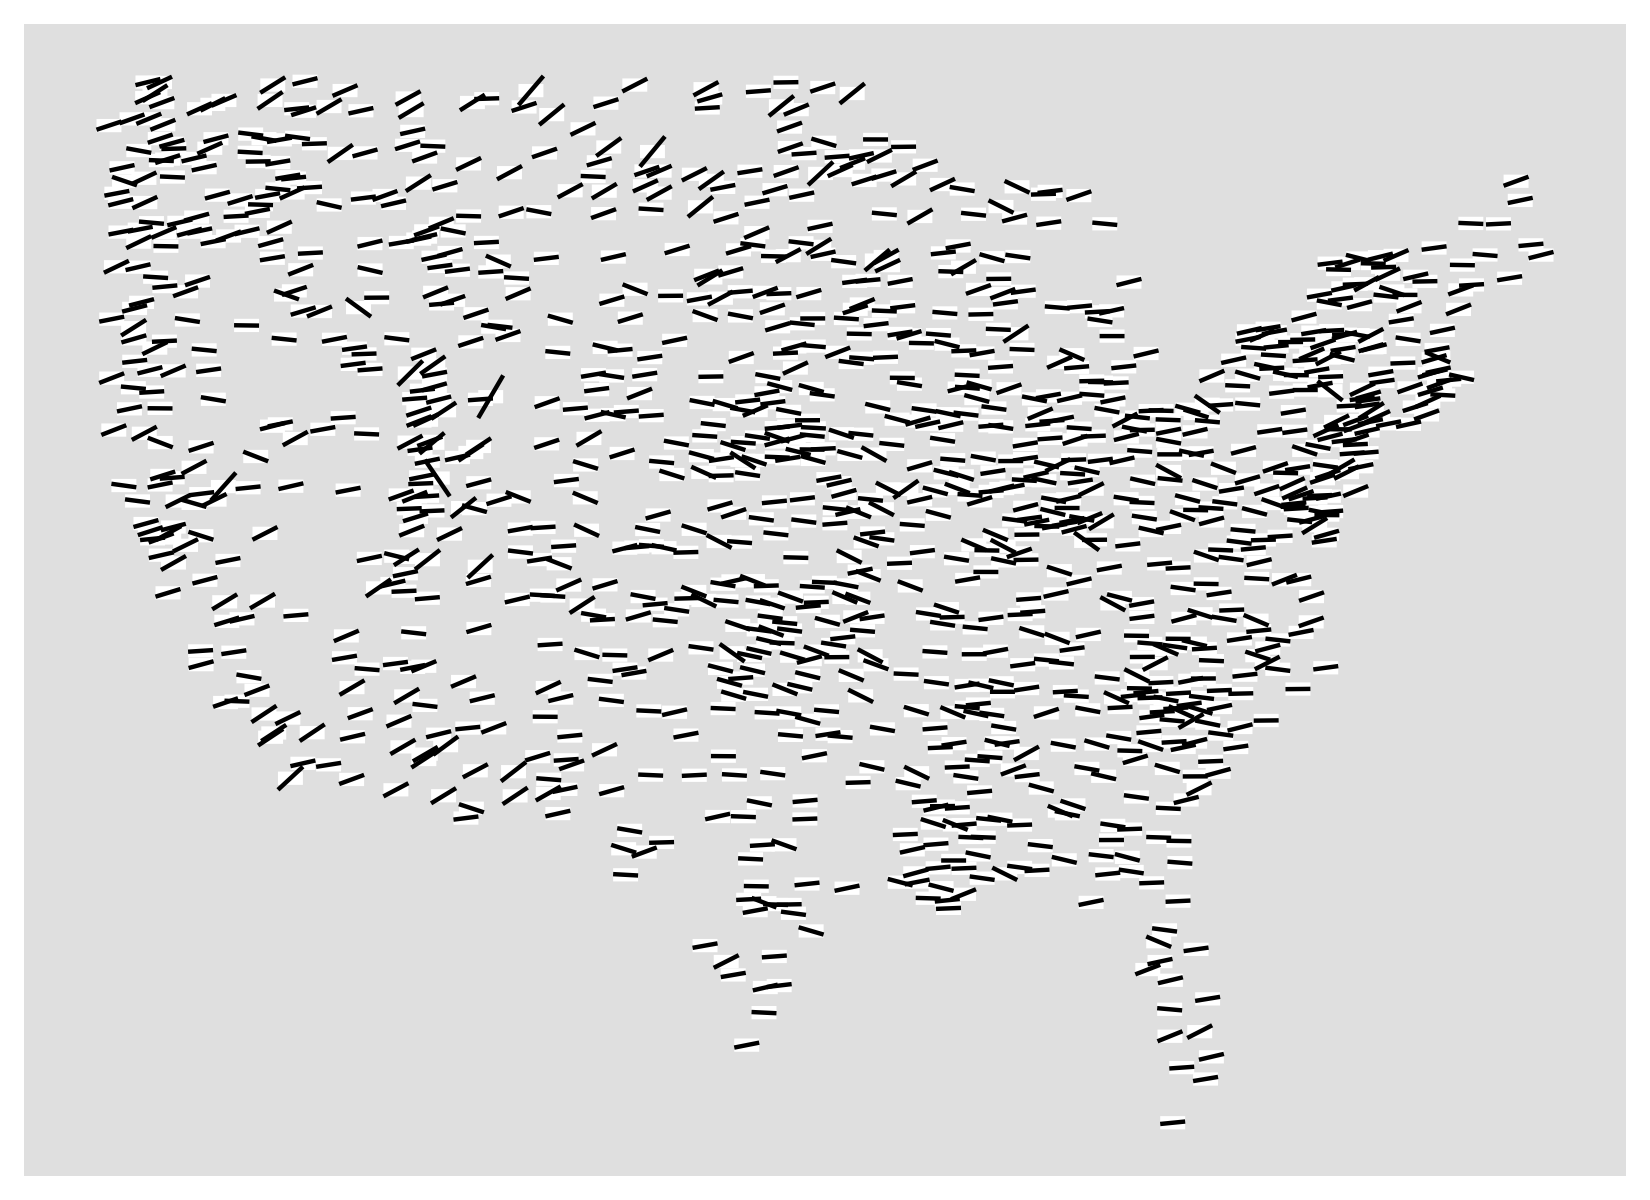
\includegraphics[width=0.55\linewidth]{usa-lin-overlap}%
  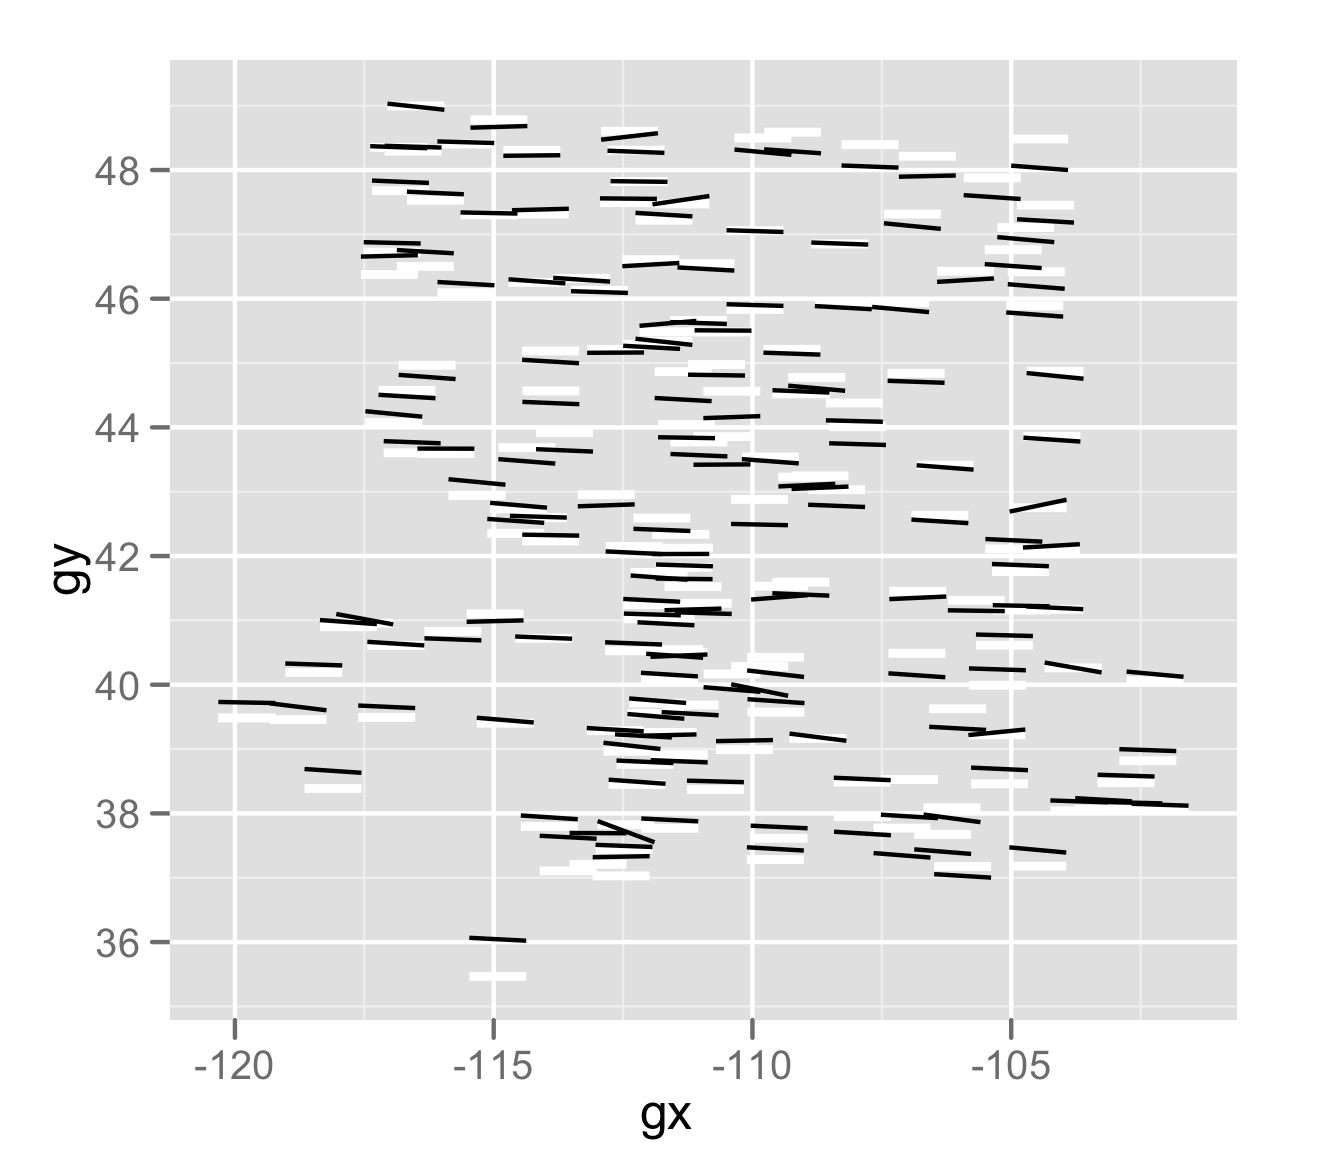
\includegraphics[width=0.35\linewidth]{ghcn-mountains}%
  \caption{Glyph-maps of the linear trend in ground station temperature values, 1950-2010, of all continental US USHCN stations (left) and stations in the mountain states (right).} 
  \label{fig:irregular}
\end{figure}
The two panels illustrate one approach to the overlapping problem: zooming.  There is an interplay between icon size (in geographical units), plotting area (in geographical units) and plot size (in display units).  Icons need to be big enough to be readable on the display, but small enough to avoid overlapping.  Readability can be maintained and overlapping reduced by decreasing the icon size and simultaneously increasing the display size or decreasing the plotting area (as done in the right panel in Figure \ref{fig:irregular}).  However, there are generally limitations in the maximum display size (or resolution) and the utility of plotting very small areas.  

An alternative approach is to combine overlapping locations and plot a single summary icon.  In Figure \ref{fig:irregular-collapsed} nearby locations are collapsed to a single icon.  In the left panel each station still has an individual glpyh but locations close to each other share a plotting area.  Not all glyphs are suited to this kind of space sharing, another option is to perform a summary of the locations that are collapsed and display that instead of the raw data.  The right panel shows an example of this where the average trend for the collapsed locations is displayed.  It is helpful to differentiate glyphs that involve summaries of more than one location, here a heavier line indicates at least two locations have been averaged.

\begin{figure}[htbp]
  \centering
  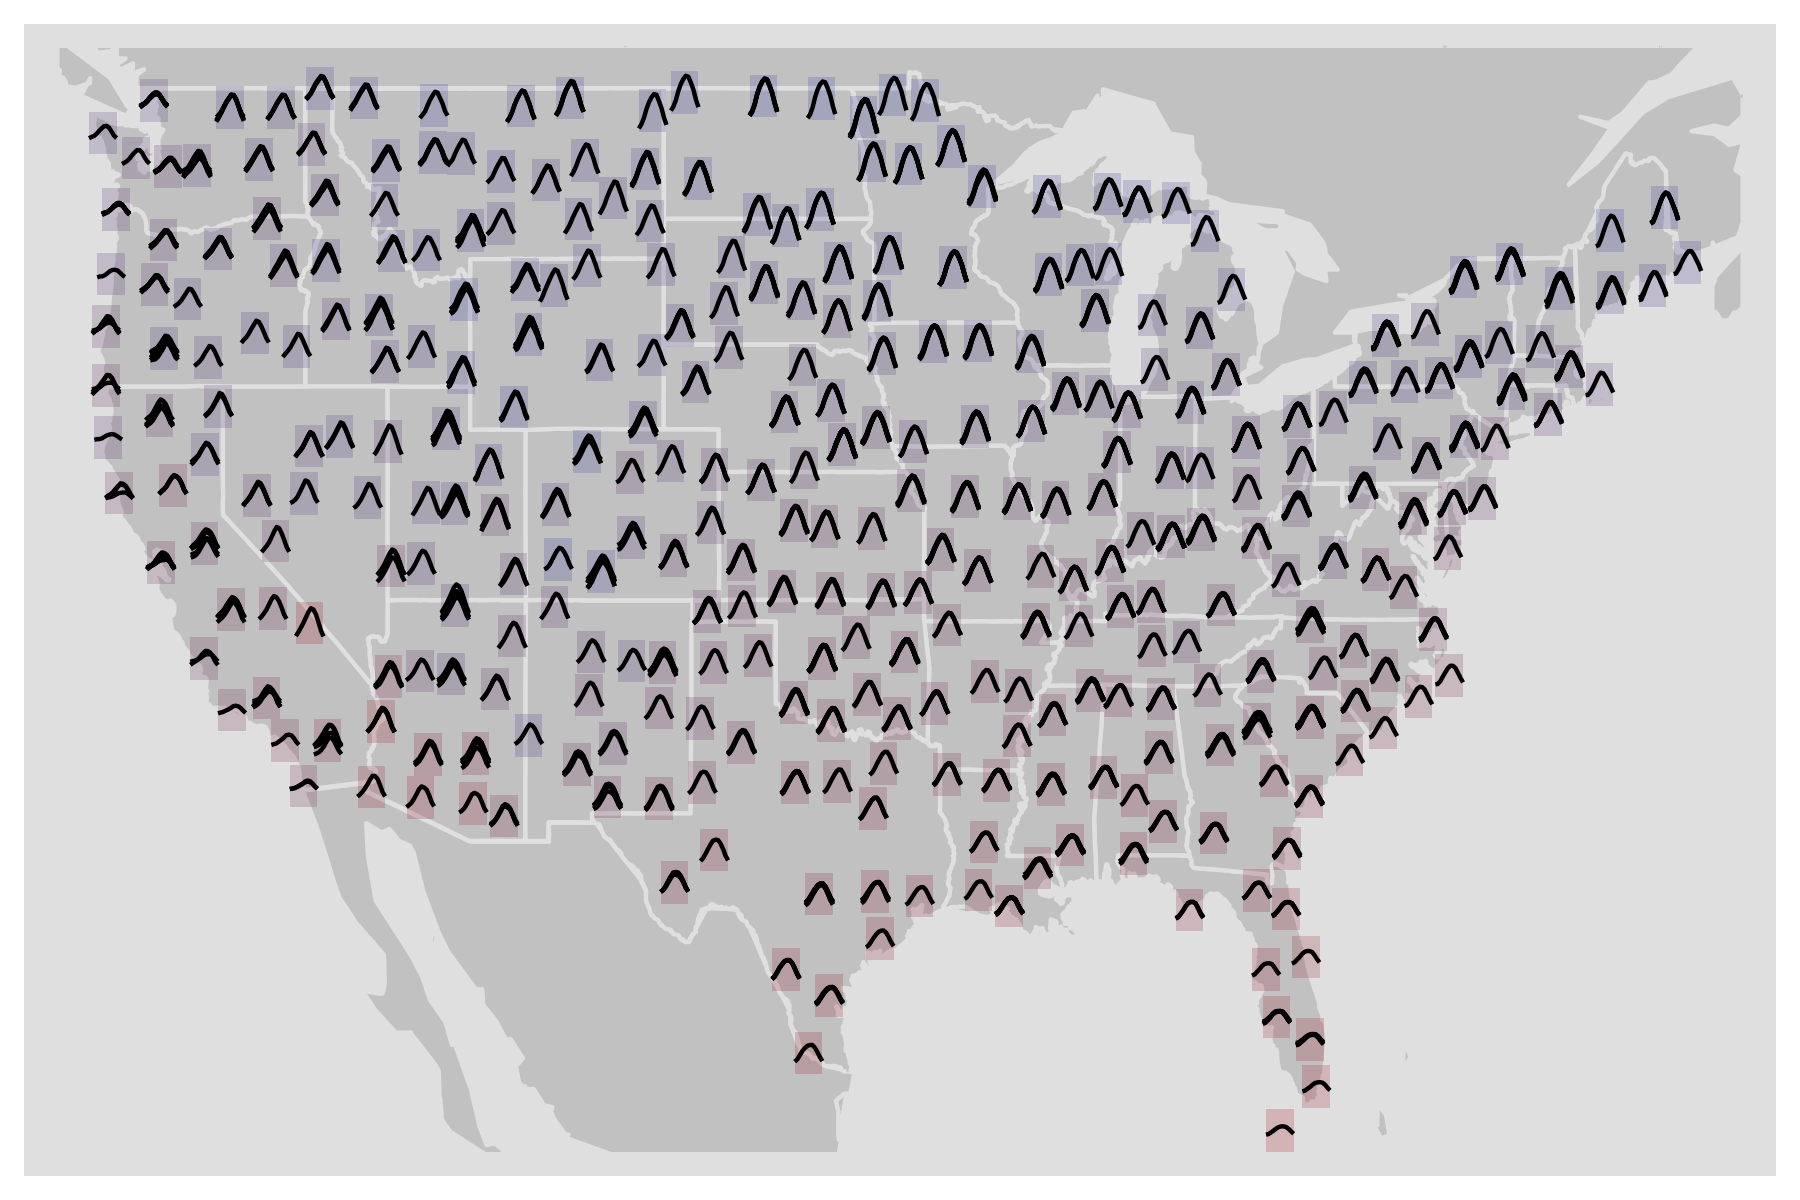
\includegraphics[width=0.5\linewidth]{usa-season-collapsed}%
  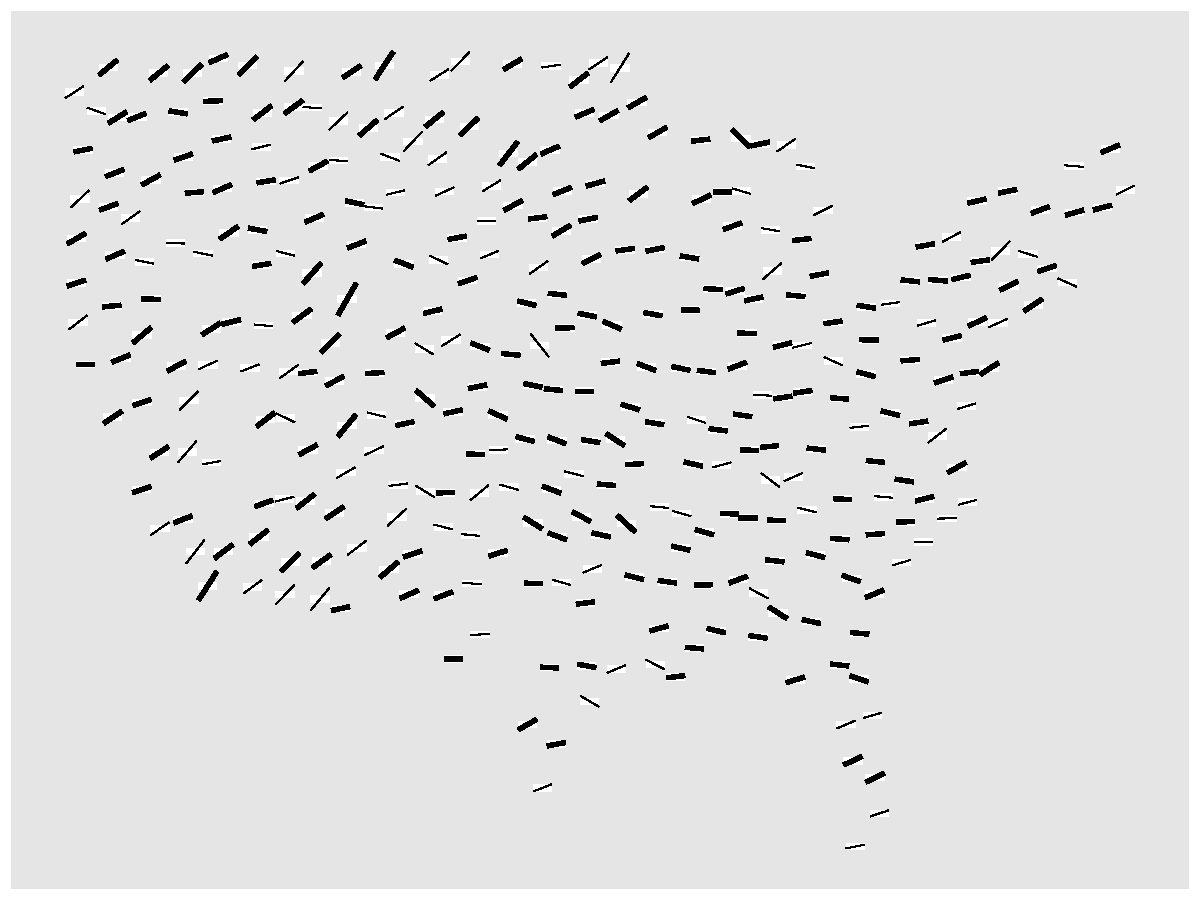
\includegraphics[width=0.5\linewidth]{usa-lin-collapse}%
  \caption{Glyph-maps of ground station temperature values, with nearby locations collapsed.1950-2010.}
  \label{fig:irregular-collapsed}
\end{figure}

In both examples of collapsing locations, the icon locations still represent real geographical locations of data, but contain data from up to an icon width away.  An alternative way to combine stations is to round locations to the icon size.  This produces a regular grid with the advantage of easier perception of structure.  However, it hides the irregular nature of the locations and icons may end up centered over nonsense places (i.e. land measurements in the ocean).

Reference guides become especially important in the irregular location case. Comparisons are harder in this case, as the ability to easily compare icons along a common baseline, be it along a row or column of glyphs, is absent. Without reference it is hard to tell if short series are missing data at the start or end.  

\section{Long time series}

A lot of climate data records contain long temporal history. For temperature records often extend from the 1800s to present day. This places some difficulties, one being computational because of the volume of records, and the second being visual display of a lot of data. Plotting the full raw time series in miniature for the glyph-maps often reveals little more than an irrelavant observation that ``temperature is quite varied!'' Careful use of de-seasonalizing, and models that can reflect nuances in global trend are needed to improve the visualization. And efficient computation to calculate and store predicted values will be required.

\section{Conclusions}

\section*{Acknowledgements}

GISTEMP data provided by the NOAA/OAR/ESRL PSD, Boulder, Colorado,
USA, from their web site at \url{http://www.esrl.noaa.gov/psd/}.

The graphics in this paper were created in R \citep{R} using {\tt ggplot2} \citep{me:ggplot2} and {\tt plyr} \citep{me:plyr}. 

\bibliography{references}

\end{document}